\chapter{Optimierung weiterer Parameter}
\label{chap:optimierung_parameter}
Grundlegend kann die Parameteruntersuchung wie eine Art Entscheidungsbaum aufgefasst werden. Dabei führt jede Entscheidung im Baum zu einer neuen Untersuchung und zu neuen Erkenntnissen. Im Verlaufe dieser Untersuchung werden somit Konzepte, Flugzustände, Komponenten und Konfigurationen ausgewählt und intensiver betrachtet. Zuerst wird eine Multicopter-Referenzkonfiguration in Kap. \ref{sec:multicopter_referenzkonfig} definiert. Danach folgt die Untersuchung einzelner Parameter auf die Flugleistungen der Referenzkonfiguration (vgl. Kap. \ref{sec:einfluss_multicopter_referenzkonfiguration}). Schließlich wird noch eine optimale Lösung vorgeschlagen und der Einfluss der AEROMET\_UAV-Randbedingungen auf diese genauer betrachtet (vgl. Kap. \ref{sec:otimale_lsg}).\\
In der folgenden Parameteruntersuchung sei nochmal auf den Aufbau der Leistungsberechnung verwiesen, der dem eines realen Systems in umgekehrter Weise gegenübersteht (Kap. \ref{sec:flugleistungsberechnung}).


\section{Multicopter-Referenzkonfiguration}
\label{sec:multicopter_referenzkonfig}
Im Folgenden soll analog zum Flächenflugzeug eine Referenzkonfiguration für einen Multicopter in Tab. \ref{tab:referenzkonfiguration_mulitcopter} festgelegt werden. Die gewählte Konfiguration ergibt sich aus vorangegangenen Untersuchungen sowie Erfahrungswerten. 

\begin{center}
	\captionof{table}{wichtige Parameter der Multicopter-Referenzkonfiguration}
	\begin{tabular}{l l l} \hline
		Parameter & Variablenname & verwendete Größe \\ \hline
		Gesamtmasse \ensuremath{m} & \texttt{m} & \SI{3,078}{kg} \\
		Leermasse des Multicopters \ensuremath{m_{copter}}& \texttt{m\_copter} & \SI{1.028}{kg} \\ 
		Batteriemasse \ensuremath{m_{Bat}} & \texttt{m\_Bat} & \SI{1,626}{kg} \\
		Motormasse \ensuremath{m_{Mot}}& \texttt{m\_Mot} & \SI{106}{g} \\
		Geschwindigkeitskonstante \ensuremath{K_V} & \texttt{K\_V} & \SI{1390}{RPM/V} \\
		maximaler Dauerstrom \ensuremath{I_{max}} & \texttt{I\_max} & \SI{35}{A} \\
		Propeller & \texttt{prop\_name} & 11x3 \\
		Anzahl Propeller \ensuremath{n_{Prop}} & \texttt{n\_prop} & \SI{4}{} \\ 
		Anzahl der Batteriezellen \ensuremath{N_{Bat,cell}} & \texttt{N\_bat\_cell} & 6 \\	 
		Obere Stirnfläche \ensuremath{F_{copter,oben}} & \texttt{F\-copter\_oben} & \SI{0,0209}{m^2} \\
		Oberer Widerstandsbeiwert \ensuremath{c_{W,copter,oben}} & \texttt{c\_W\_copter\_oben} & 1 \\ \hline
	\end{tabular}	
	\label{tab:referenzkonfiguration_mulitcopter}
\end{center}

Die Umgebungsparameter sind die für eine Standardatmosphäre auf Meereshöhe (entspr. QNH). Dazu wurde der Seitenwind nicht wie im AEROMET\_UAV Projekt auf \SI{100}{km/h} sondern auf konstante \SI{10}{m/s} festgesetzt. Der Grund hierfür ist, dass der Leistungsüberschuss in einem mäßig schnellen Vorwärtsflug am größten ist \cite[S.328-S.329]{Wall.2015}. Dieser Zusammenhang wird mit der Windgeschwindigkeit modelliert. Außerdem kann der Einfluss einzelner Parameter besser und genauer untersucht werden. Die AEROMET\_UAV Randbedingungen werden später in Abschn. \ref{subsec:aeromot_rb} berücksichtigt.

\section{Einflussfaktoren auf die Multicopter-Referenzkonfiguration}
\label{sec:einfluss_multicopter_referenzkonfiguration}
Für einen Multicopter gibt es viele Einflussfaktoren, die im Folgenden genauer betrachtet werden sollen.

\subsection{Einfluss des Luftwiderstands}
\label{subsec:widerstandseinfluss}
Der Widerstandsbeiwert hat einen Einfluss auf die Flugleistungen eines Multicopters, der als gering eingeschätzt werden kann (vgl. Abb. \ref{abb:c_W_einfluss}). Unabhängig von dem Widerstandsbeiwert \ensuremath{c_W} endet für alle Konfigurationen der Steigflug bei der Dienstgipfelhöhe. Auch hier stellt die Prepellerdrehzahl den die Höhe limitierenden Parameter dar, die ab \SI{20100}{RPM} eine Blattspitzengeschwindigkeit \ensuremath{Ma_{tip}} von \ensuremath{Ma = 1} erreicht. Das Erreichen der Dienstgipfelhöhe wirkt sich jedoch kaum auf die Restladung aus.\\
Bis zu einer Höhe von \SI{15000}{m} erfolgt der Steigflug bei maximalen Motorstrom \ensuremath{I_{max}}. Mit dem Schub und der abnehmenden Dichte steigt die Drehzahl, die in einer Erhöhung der Motorspannung mündet. Durch die Belastung fällt die Batteriespannung ab, sodass diese in Kombination mit der Motorspannung in einer PWM Erhöhung resultiert. Nach einem anfänglichen Anstieg auf ca. \SI{52,5}{\%} fällt der Gesamtwirkungsgrad \ensuremath{\eta_{ges}} auf \SI{41,5}{\%} ab. 
Am deutlichsten kann der Einfluss des Widerstandsbeiwertes an dem Verlauf der Restladung und der Bahngeschwindigkeit ausgemacht werden. 
Bei einem großen maximalen Motorstrom gilt, dass die Begrenzung der Geschwindigkeit durch den Widerstandsbeiwert erfolgt. Eine sehr hohe Geschwindigkeit verringert zum einen die Flugzeit für einen Höhenschritt, erhöht auf der anderen Seite jedoch den Widerstand und damit zusätzlich die benötigte Leistung (vgl. Gleichung \eqref{eq:widerstand}). Je geringer der \ensuremath{c_W}-Wert gewählt wird, desto höher ist die optimale Bahngeschwindigkeit. Erhöht sich im Umkehrschluss der Luftwiderstand so sinkt die Bahngeschwindigkeit, da der Widerstand mit der Geschwindigkeit quadratisch (vgl. Gleichung \eqref{eq:widerstand}) ansteigt. Zudem erhöht ein geringer Widerstandsbeiwert die vorhandene Restkapazität. Anhand der Restkapazitätsabnahme kann ein beinahe lineare Abhängigkeit zwischen einer \ensuremath{c_W}-Erhöhung und einer Abnahme der Restladung festgestellt werden. Im Schnitt sinkt mit einer Anhebung des \ensuremath{c_W}-Wertes um 0,5 die Restladung auf \SI{15000}{m} um \SI{4}{\%}. Im Vergleich zum Einfluss der Gleitzahl auf die Flugleistungen eines Flächenflugzeuges ist der Verlauf hier ähnlich (vgl. Abb. \ref{subsec:gleitzahl}). 
Im Sinne einer großen maximalen Höhe ist daher eine aerodynamisch günstige Verkleidung des Multicopters anzustreben.
  
\begin{figure}[H]
\centering
	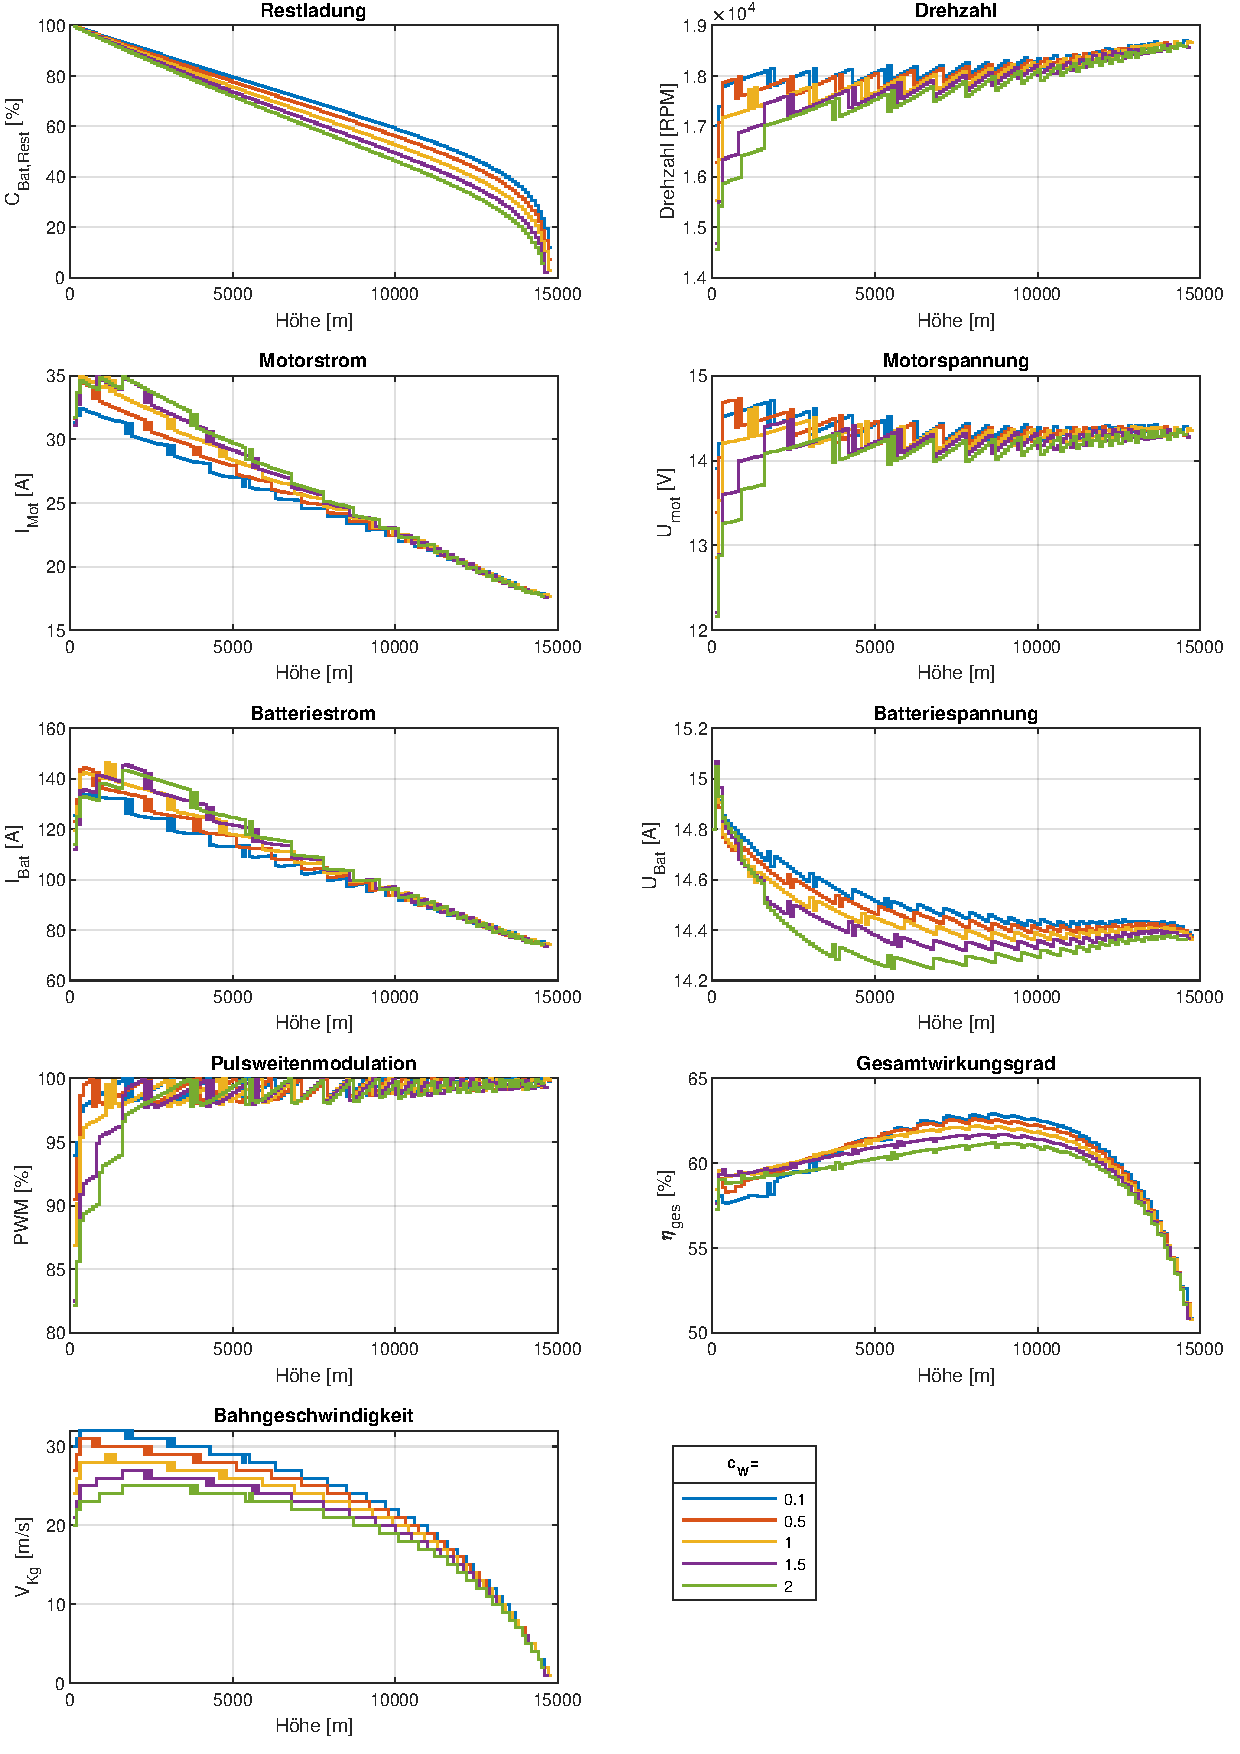
\includegraphics[scale=0.7]{Diagramme/Untersuchung_c_W.pdf}
	\caption{Einfluss des Widerstandsbeiwertes auf die Flugleistungen der Multicopter-Referenzkonfiguration (Tab. \ref{tab:referenzkonfiguration_mulitcopter})}
	\label{abb:c_W_einfluss}
\end{figure}


\subsection{Einfluss der Batteriespannung}
\label{subsec:einfluss_n_bat}
Wie in Kap. \ref{subsec:mot_prop_kombi} gezeigt, ist ein weiterer begrenzender Parameter die max. Motorleistung bzw. die PWM. Die Motorspannung an sich kann nicht beeinflusst werden. Jedoch lässt sich Einfluss auf die Höhe der Motorspannung durch eine Erhöhung der in Reihe geschalteten Batteriezellen nehmen. Mit jeder zusätzlichen Zelle erhöht sich die nominelle Batteriespannung um \SI{3,7}{V} (vgl. Abb. \ref{abb:N_Bat_einfluss}). Damit stellt die PWM nicht mehr die Grenze für die Bahngeschwindigkeit dar. Der effizienteste Flugzustand ist nun der beim maximalen, dauerhaften Motorstrom. Jedoch führt bei gleicher Energiemenge und somit gleicher Masse 
\begin{equation}
	E_{Bat} = C_{Bat}\cdot U_{Bat}
\end{equation}
eine Erhöhung der Spannung in dem Produkt aus Spannung und Kapazität (\ensuremath{C_{Bat} = I_{Bat}\cdot t_{Flug}}) unweigerlich zu einer Verringerung der Kapazität.  \\
Alle Batteriekonfigurationen steigen bis zu ihrer Dienstgipfelhöhe auf. 
Für die Batterie mit nur zwei Zellen ist diese durch die PWM bei \SI{100}{\%} bereits kurz nach Beginn des Steigfluges erreicht. Der Grund dafür ist der aufgebrauchte Leistungsüberschuss. Die Motorspannung ist durch die Batteriespannung (und die PWM) begrenzt, weshalb die Propellerdrehzahl auch begrenzt ist. Folglich ist der Schub beschränkt, was zu einer Abnahme der Bahngeschwindigkeit auf \SI{0}{m/s} führt. \\
Deutlich bessere Ergebnisse liefert eine Verdoppelung der Zellenanzahl auf vier. Diese Konfiguration erreicht auch die Dienstgipfelhöhe, jedoch ist das Niveau der nominellen Batteriespannung im Gegensatz zu der zweizelligen Batterie doppelt so hoch. Dies bedeutet, dass zu Beginn des Fluges der Motor wieder am effizientesten mit maximalem Strom \ensuremath{I_{max}} betrieben werden kann. Im Laufe des Fluges steigt die Drehzahl des Propellers und somit die auch die Motorspannung (vgl. Gleichung \eqref{eq:motorspannung}). Dieser Betriebszustand ist wieder solange möglich bis kein Leistungsüberschuss mehr vorhanden ist und die PWM \SI{100}{\%} erreicht. Es kommt zu einer Limitierung der Drehzahl durch die Motorspannung und letztendlich zum immer schneller werdenden Absinken der Bahngeschwindigkeit. \\
Die Leistungsparameter für die Batterien mit mehr als vier Zellen in Reihe sind in Bezug auf die Restladung die Propellerdrehzahl, den Motorstrom und die -spannung sowie die Bahngeschwindigkeit beinahe identisch. Lediglich in den Batteriekenngrößen und damit auch in der PWM treten Unterschiede auf, weil mit der Zellenanzahl die nominelle Batteriespannung steigt und damit die PWM sinkt (vgl. Gleichung \eqref{eq:pwm}). Der Batteriestrom nimmt ebenfalls durch die sinkende PWM ab. Die Dienstgipfelhöhe ist analog zu Abschn. \ref{subsec:widerstandseinfluss} durch die maximale Propellerdrehzahl und diese wiederum durch die Blattspitzengeschwindigkeit begrenzt. \\
Ein Optimum für die günstigste Anzahl an Batteriezellen liegt bei \ensuremath{N_{Bat,cell} = 4} vor, da diese Konfiguration in jedem Höhenschritt die größte Restladung aufweist (vgl. Abb. \ref{abb:N_Bat_einfluss}). Dies ist jedoch einzuschränken. Diese Konstellation erreicht die geringste Abnahme der Restkapazität mit der Höhe, jedoch schränkt die im Vergleich zu Batterien mit mehr Zellen geringere, nominelle Batteriespannung die Motorleistung ein, was zu einem frühzeitigen Beenden des Steigflugs durch Erreichen der Dienstgipfelhöhe führt. Dieser Flaschenhals ist bei mindestens einer Zelle mehr nicht mehr gegeben. In diesem Sinne ist eine fünfzellige Batterie für die Multicopter-Referenzkonfiguration zu bevorzugen. Jedoch weist die vierzellige Batterie den größten Gesamtwirkungsgrad auf. Dieser fällt ebenfalls mit der nominellen Batteriespannung. Insbesondere für die Batterien mit mehr als vier Zellen sind der Propeller- und Motorwirkungsgrad identisch, da die Leistungsgrößen, die auf diese Wirkungsgrade einen Einfluss haben, ebenfalls identisch sind. \\
Der Grund für die unterschiedlichen Gesamtwirkungsgrade liegt im Wirkungsgrad des Motorreglers. Eine sinkende PWM erhöht die Verluste innerhalb der Motorregler und verringert den Wirkungsgrad (vgl. Gleichung \eqref{eq:eta_pwm}). Dies soll in Abschn. \ref{subsec:einfluss_eta_pwm} genauer untersucht werden.\\
Insgesamt ist für die Batteriezellenanzahl ein Kompromiss zu wählen. 
Mehr in Reihe geschaltete Batteriezellen erhöhen wie bereits erwähnt die nominelle Batteriespannung. Somit stellt die Motorleistung nicht mehr den limitierenden Parameter dar. Auf der anderen Seite ist die verfügbare Leistung am Motoreingang so hoch, dass sie bei vollständiger Nutzung (\SI{100}{\%} PWM) und einer Luftdichte in Bodennähe zum Überschreiten des maximal zulässigen Motorstroms führt. Folglich ist eine Regulierung der PWM zwingend erforderlich. Diese Regulierungsgrenze verschiebt sich in Bezug zur PWM weiter nach unten, je größer die nominale Batteriespannung ist. Damit steigen auch die Motorreglerverluste.

\begin{figure}[hbt!]
\centering
	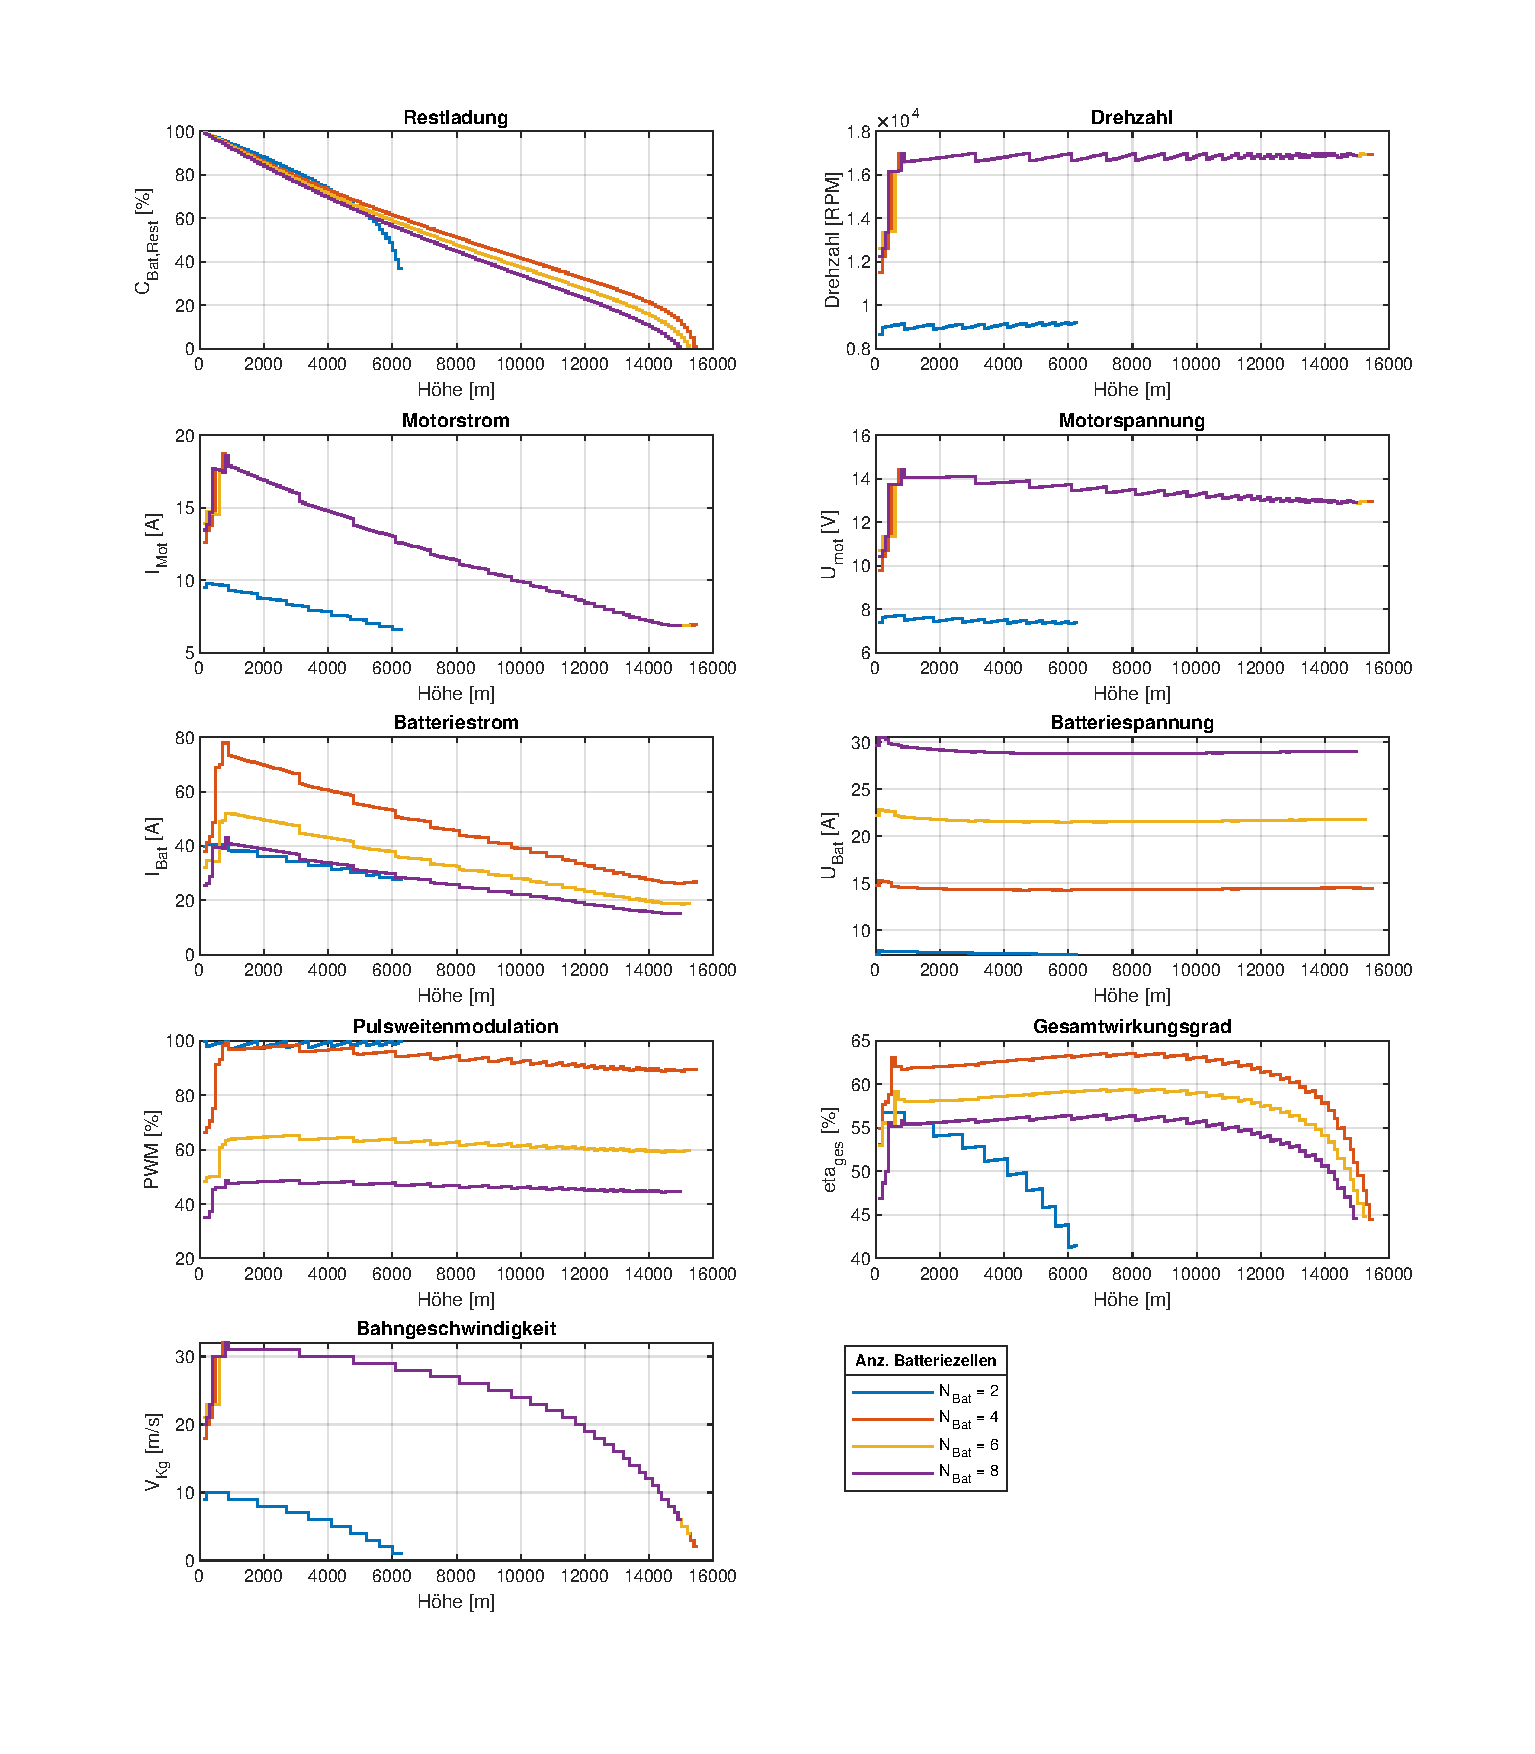
\includegraphics[scale=0.70]{Diagramme/Untersuchung_N_Bat.pdf}
	\caption{Einfluss des Batteriezellenanzahl auf die Flugleistungen der Multicopter-Referenzkonfiguration (Tab. \ref{tab:referenzkonfiguration_mulitcopter})}
	\label{abb:N_Bat_einfluss}
\end{figure}


\subsection{Einfluss des Motorreglerwirkungsgrades}
\label{subsec:einfluss_eta_pwm}
Der Wirkungsgrad des ESC ist ausschließlich als eine Funktion der PWM modelliert (vgl. Gleichung \eqref{eq:eta_pwm}). Wie bereits in Abschn. \ref{subsec:einfluss_n_bat} erklärt, sinkt die PWM mit der Erhöhung der Batteriezellenanzahl. Zeitgleich steigen die Verluste im Motorregler. Im Sinne eines besseren Gesamtwirkungsgrades und der erreichbaren Höhe ist eine Verringerung der Motorreglerverluste anzustreben. Die Ergebnisse sind in \ref{sec:motorreglerwirkungsgrad} dargelegt. \\
Der Motorreglerwirkungsgrad hat keinen Einfluss auf die Dienstgipfelhöhe. Es ist allerdings ein bedeutender Einfluss auf die Restladung zu erkennen. Mit einem höheren ESC-Wirtkungsgrad steigt auch der Gesamtwirkungsgrad. Weiterhin sinkt der Batteriestrom (vgl. Gleichung \eqref{eq:batteriestrom}) mit dem Reglerwirkungsgrad und über den geringeren Batteriestrom sinkt die der Batterie entnommene Kapazität. Werden die Kurven der Restladung linear extrapoliert, so würde die Konfiguration mit sechs Zellen und bei einer Halbierung der Verluste im Motorregler ohne die Dienstgipfelhöhe bereits \SI{18000}{m} und mit keinen Verlusten im Regler bereits mehr als \SI{20000}{m} Höhe erreichen. \\
Daher sind aus den oben genannten Gründen die Verluste innerhalb des Motorreglers zu verringern. 


\subsection{Einfluss des maximalen Motorstroms}
\label{subsec:einfluss_imax}
Die Ergebnisse zeigen, dass ein geringer maximaler Motorstrom ebenfalls die Bahngeschwindigkeit begrenzt (vgl. z.B. Abb. \ref{abb:c_W_einfluss}). Dieser begrenzt die dem Motor entnommene Leistung. 
Folglich ist ein Motor für einen solchen Steigflug zu wählen, der einerseits einen hohen \ensuremath{K_V}-Wert besitzt, andererseits aber auch einen hohen maximalen Dauerstrom besitzt (vgl. Kap. \ref{subsec:mot_prop_kombi}). Ein gutes Beispiel ist der Motor aus Kapitel \ref{sec:flaechenflugzeug_referenzkonfig} mit einem \ensuremath{K_V}-Wert von \SI{1390}{RPM/V} und einem maximalen Motorstrom \ensuremath{I_{max}} von \SI{35}{A}.



%******************************************************************

\subsection{Massenanteile der Komponenten}
\label{subsec:massenverteilung}
Ein weiterer wichtiger Punkt, der an dieser Stelle untersucht werden soll, ist die Massenanteilsverteilung von den Motoren, der Batterie und der Leermasse des Multicopters am Gesamtgewicht. Wiederum stellt der Quadrocopter aus Kapitel \ref{chap:nachbildung_des_quadrocopter} die Grundlage der Untersuchung dar. Bei diesem nehmen die Motoren \SI{13,77}{\%}, die Batterie \SI{52,83}{\%} und der Rahmen mit den übrigen Komponenten \SI{33,4}{\%} der Gesamtmasse von \SI{1060}{g} ein. Diese Massenverhältnisse sind bereits bei der Multicopter-Referenzkonfiguration angewendet worden (vgl. Kap. \ref{sec:multicopter_referenzkonfig}). Zusätzlich wurde auch die obere Stirnfläche \ensuremath{F_{copter,oben}} mit der Größe angepasst. Für die genauere Betrachtung der optimalen Massenverteilung wird die Batteriemasse im Verhältnis zur Gesamtmasse variiert.

\begin{figure}[H]
\centering
	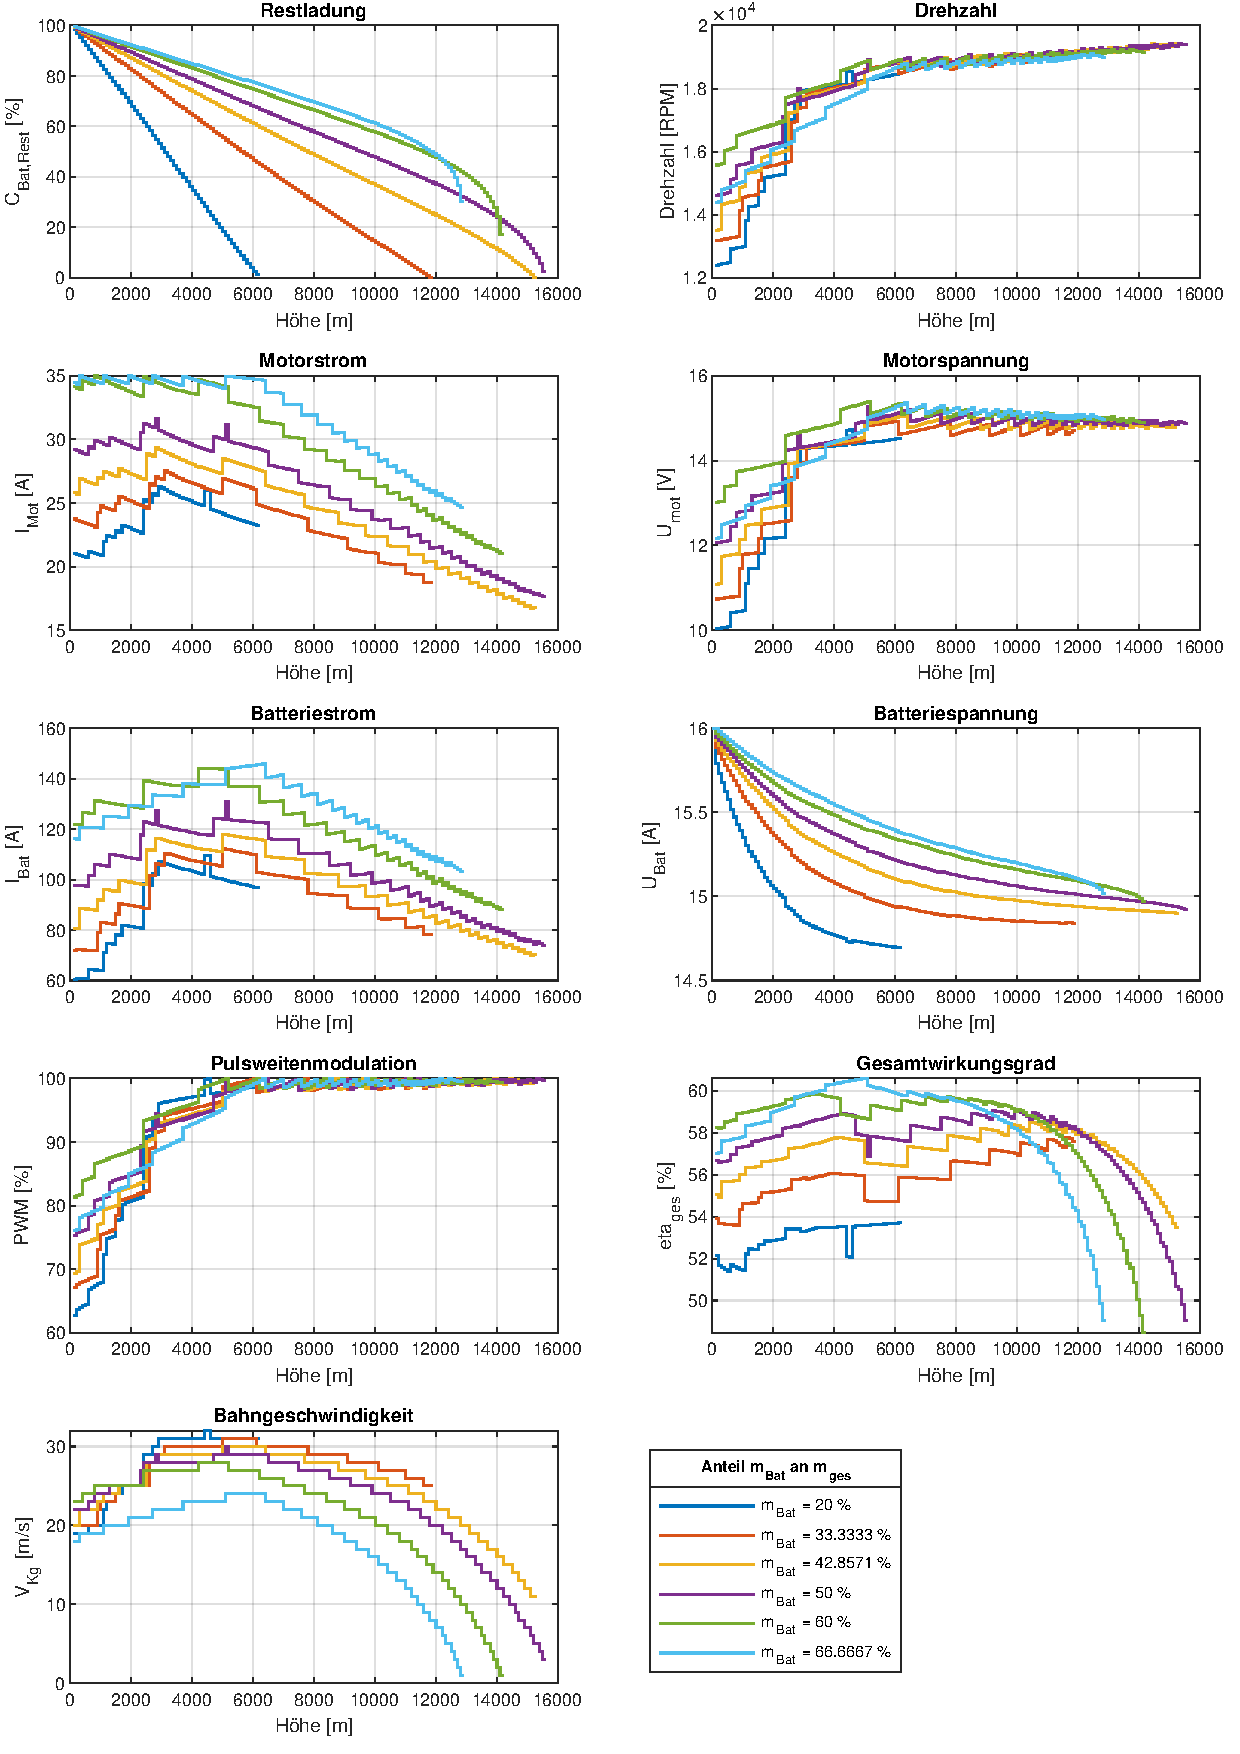
\includegraphics[scale=0.70]{Diagramme/Batteriemasse.pdf}
	\caption{Einfluss des Batteriemassenanteils auf die Flugleistungen der Multicopter-Referenzkonfiguration (Tab. \ref{tab:referenzkonfiguration_mulitcopter})}
	\label{abb:batteriemasse}
\end{figure}

Der Einfluss der Batteriemasse auf die Flugleistungen ist bedeutend (vgl. Abb. \ref{abb:batteriemasse}). Die TOCs variieren in eine Spanne von \SI{5000}{m}. Hier kommt es zu einer Überlagerung zweier Effekte. Der erste ist der Einfluss der Batteriezellenanzahl, der bereits in Abschn. \ref{subsec:einfluss_n_bat} genauer erklärt wurde, und der zweite ist der Einfluss der Batteriemasse. \\
Es kann festgehalten werden, dass mit der Batteriemasse die Batteriekapazität steigt (vgl. Gleichung \eqref{eq:batteriekapazitaet}). Die zur Verfügung stehende Energie erhöht sich. Außerdem erhöht eine höhere Batteriemasse die Gesamtmasse (vgl. Gleichung \eqref{eq:masse_multicopter}) und als Konsequenz auch den erforderlichen Propellerschub (vgl. Gleichung \eqref{eq:neigungswinkel} und \eqref{eq:schub_multicopter}). Diesem folgt eine Erhöhung des Motor- (vgl. Gleichung \eqref{eq:motorstrom}) und des Batteriestroms (vgl. \eqref{eq:batteriestrom}).
Bei Batteriemassenanteilen von weniger als \SI{33,33}{\%}, also einem Drittel der Gesamtmasse, limitiert die Batteriekapazität den Steigflug. Durch die geringe Masse werden die Motoren nicht vollständig ausgelastet, sodass der Motorstrom mit dem Drehmoment des Propellers kontinuierlich ansteigt (vgl. Gleichung \eqref{eq:motorstrom}). Der Drehzahlzuwachs ist zudem signifikant größer als bei höheren Batteriemassenanteilen. Entsprechend steigt auch die Motorspannung an (vgl. Gleichung \eqref{eq:motorspannung}). Der Batteriestrom nimmt äquivalent zum Motorstrom und -spannung zu (vgl. Gleichung \eqref{eq:batteriestrom}).
Zudem ist ein stärkerer Spannungseinbruch zu verzeichnen, je kleiner der Batteriemassenanteil ist. Eine Erklärung liefert die Entladerate, die sich aus dem Batteriestrom in Abhängigkeit der Kapazität zusammensetzt und für eine geringere Kapazität steigt (vgl. Gleichung \eqref{eq:c_rate}). Die Bahngeschwindigkeit ist jedoch am höchsten und sinkt mit höherem Gesamtgewicht, weil der Schub und letztlich die notwendige Energie mit dem Gewicht und der Bahngeschwindigkeit steigen. Weiterhin kann die Dienstgipfelhöhe durch die Motorleistung nicht erreicht werden. Bei sehr kleinen Batterien reicht hierzu die Kapazität nicht aus. Deshalb kann der volle Leistungsüberschuss nicht genutzt werden. \\
Anders ist dies, wenn die Batterie die Hälfte der Gesamtmasse ausmacht. Auch hier limitiert die Batteriekapazität die Flughöhe. Jedoch ist die absolute Kapazität bedeutend höher, weshalb auch die maximale Flughöhe höher ist. Wiederum kann der Einfluss der Batteriezellenanzahl auf Batterien mit der gleichen Masse und Kapazität beobachtet werden. Dieser Zusammenhang wird in Abschn. \ref{subsec:einfluss_n_bat} genauer beschrieben. Ab dieser Batteriemasse ist wieder ein effizienter Flug mit maximalen Motorstrom möglich. Je nach der Batteriezellenanzahl ändert sich auch die Dienstgipfelhöhe. Bei \ensuremath{n_{Bat,cell} = 6} ist dies wiederum durch die maximale Propellerdrehzahl begrenzt und bei \ensuremath{n_{Bat,cell} = 4} limitiert die PWM die Motorleistung, sodass der Schubüberschuss aufgebraucht ist. Die Abhängigkeit der Flugleistungen von der Batteriezellenanzahl zeigt auch die Batterie mit einem Massenanteil von \ensuremath{2/3} an der Gesamtmasse. Hier ist die Batteriekapazität wieder größer. Dies verdeutlicht sich in der nochmals geringeren Batteriekapazitätsabnahme. Mit der Masse sinkt auch die Propellerdrehzahl. Durch die größere Gesamtmasse steigt der benötigte Standschub (vgl. Gleichung \eqref{eq:neigungswinkel} und \eqref{eq:schub_multicopter}) und damit sinkt die optimale Bahngeschwindigkeit.
%, weil die Bahngeschwindigkeit mit dem Widerstand erhöht (vgl. Gleichung \eqref{eq:widerstand}).
Zum Schluss steigert der Batteriemassenanteil noch den Gesamtwirkungsgrad. 
Ein Optimum des Batteriemassenanteils liegt bei \SI{66,667}{\%} der Gesamtmasse (vgl. Anhang \ref{sec:batteriemasse}). Dabei ist vor allem noch die Anzahl der Batteriezellen zu berücksichtigen. Im Hinblick auf Abschn. \ref{subsec:einfluss_n_bat} ist die Zellenanzahl auf den Motor anzupassen, sodass die Motorleistung die maximale Höhe nicht begrenzt, wobei der Motorregler verlustarm arbeiten sollte. Auf der anderen Seite sollte die nominelle Batteriespannung nicht so hoch sein, dass die PWM zum Schutz des Motors abgeriegelt werden muss (vgl. Abschn. \ref{subsec:einfluss_n_bat}). 
Der hier ermittelte optimale Batteriemassenanteil stimmt mit den Aussagen von Neitzke überein \cite{Neitzke.2013}.
Es ist außerdem ersichtlich, dass die Flugleistung und -dauer noch weiter verbessert werden können, wenn der Massenanteil des Rahmens und aller übriger Komponenten kleiner wird und die Masse der Batterie im Gegensatz steigt, d.h. eine Tendenz der Multicopterleermasse gegen Null (\ensuremath{m_{Copter}\rightarrow 0} und \ensuremath{m_{Bat}\rightarrow (m_{Bat}+m_{Copter})}).


%******************************************************************
\subsection{Einfluss der Größe}
\label{subsec:groesse}
Ein weitere Einfluss auf die Flugleistungen stellt das Gesamtgewicht des Fluggerätes dar. Dabei wird das Fluggerät äquivalent skaliert. Dies bedeutet, dass die Massenverhältnisse von Motoren, Batterien und die Leermasse im Verhältnis zum Gesamtgewicht konstant bleiben. Das Verhältnis orientiert sich an der Massenverteilung aus Kapitel \ref{subsec:massenverteilung}. Dieses Verhältnis wird für jede Größenskalierung gewahrt. Als Anhaltspunkt dient wieder die Motormasse. Die Propellerauswahl findet nach den Herstellerempfehlungen und eigenen Versuchen statt. Alle anderen Massenverteilungen ergeben sich im Anschluss aus der Motormasse analog zu Kapitel \ref{subsec:massenverteilung}.

\begin{figure}[H]
%\centering
	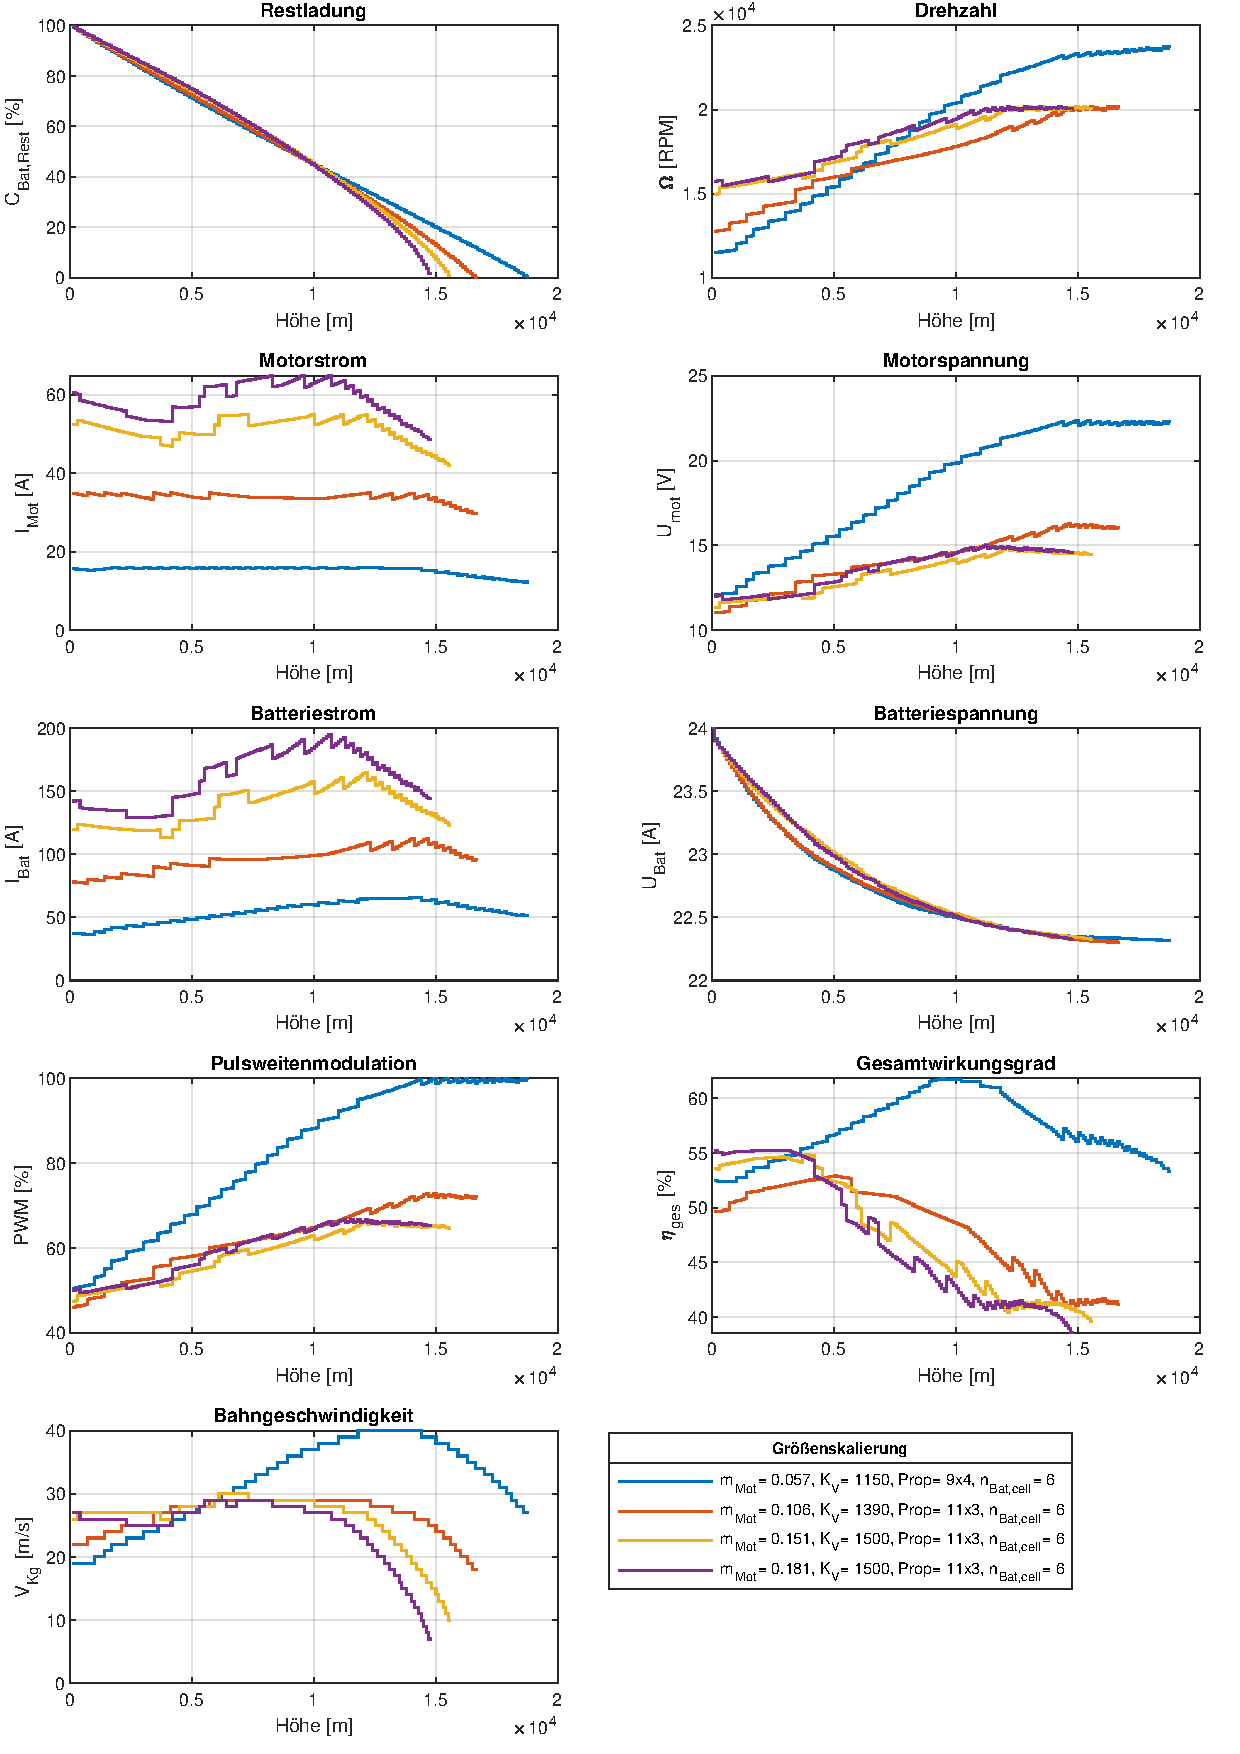
\includegraphics[scale=0.7]{Diagramme/Groessenskalierung.pdf}
	\caption{Einfluss der äquivalenten Größenveränderung auf die Flugleistungen der Multicopter-Referenzkonfiguration (Tab. \ref{tab:referenzkonfiguration_mulitcopter})}
	\label{abb:groessenskalierung}
\end{figure}
Eine äquivalente Größenskalierung besitzt einen vernachlässigbar kleinen Einfluss auf die Flugleistungen (vgl. Abb. \ref{abb:groessenskalierung}). Die Abnahme der Restladung ist für alle Konstellationen beinahe identisch. Der Grund für die Unterschiede in den Diagrammen, die vor allem die Höhe betreffen, liegt in den Unterschieden der Motoren und Propeller. Eine vollständige, uniforme Skalierung ist hier nicht möglich. Dabei unterscheiden sich besonders die \ensuremath{K_V}-Werte der Motoren. Dies zieht Unterschiede im Bereich der Motorspannung und folglich in der PWM und im Gesamtwirkungsgrad nach sich. \\
An dieser Stelle kann somit festgehalten werden, dass eine Größenskalierung keinen Einfluss auf die Flugleistungen hat. Die Vorteile einer größeren Masse liegen für reale Anwendungsfälle vorrangig in der Massenträgheit. In einem Höhensektor von \SI{0}{m} bis \SI{15000}{m} treten im Durchschnitt \SI{100}{km/h} starke Winde auf \cite{Seidel.2011}. Die Einflüsse von Böen in diesen Größenordnungen auf einen Multicopter fallen geringer aus, wenn das Fluggerätes auf eine höhere Gesamtmasse ausgelegt wird. Dies erfordert im Umkehrschluss weniger Energie zur Kurs- und Lagekorrektur. \\
Im Hinblick auf die angedachte Nutzlast von \SI{250}{g} im Rahmen des AEROMET\_UAV-Projektes bietet eine größere Gesamtmasse den Vorteil, dass die feste Masse der Nutzlast anteilig an der Gesamtmasse weniger wird, je größer die Gesamtmasse ist.


\subsection{Anzahl der Propeller}
\label{subsec:anz_prop}
% Wie sich in Abschn. \ref{subsubsec:groesse} zeigte, hat eine uniforme Skalierung des Fluggerätes keinen Einfluss auf dessen Flugleistung. 
Bisher wurden nur Fluggeräte mit vier Rotoren untersucht. Dabei gilt es noch die Abhängigkeit der Flugleistungen von der Propelleranzahl zu überprüfen. 

\begin{figure}[H]
%\centering
	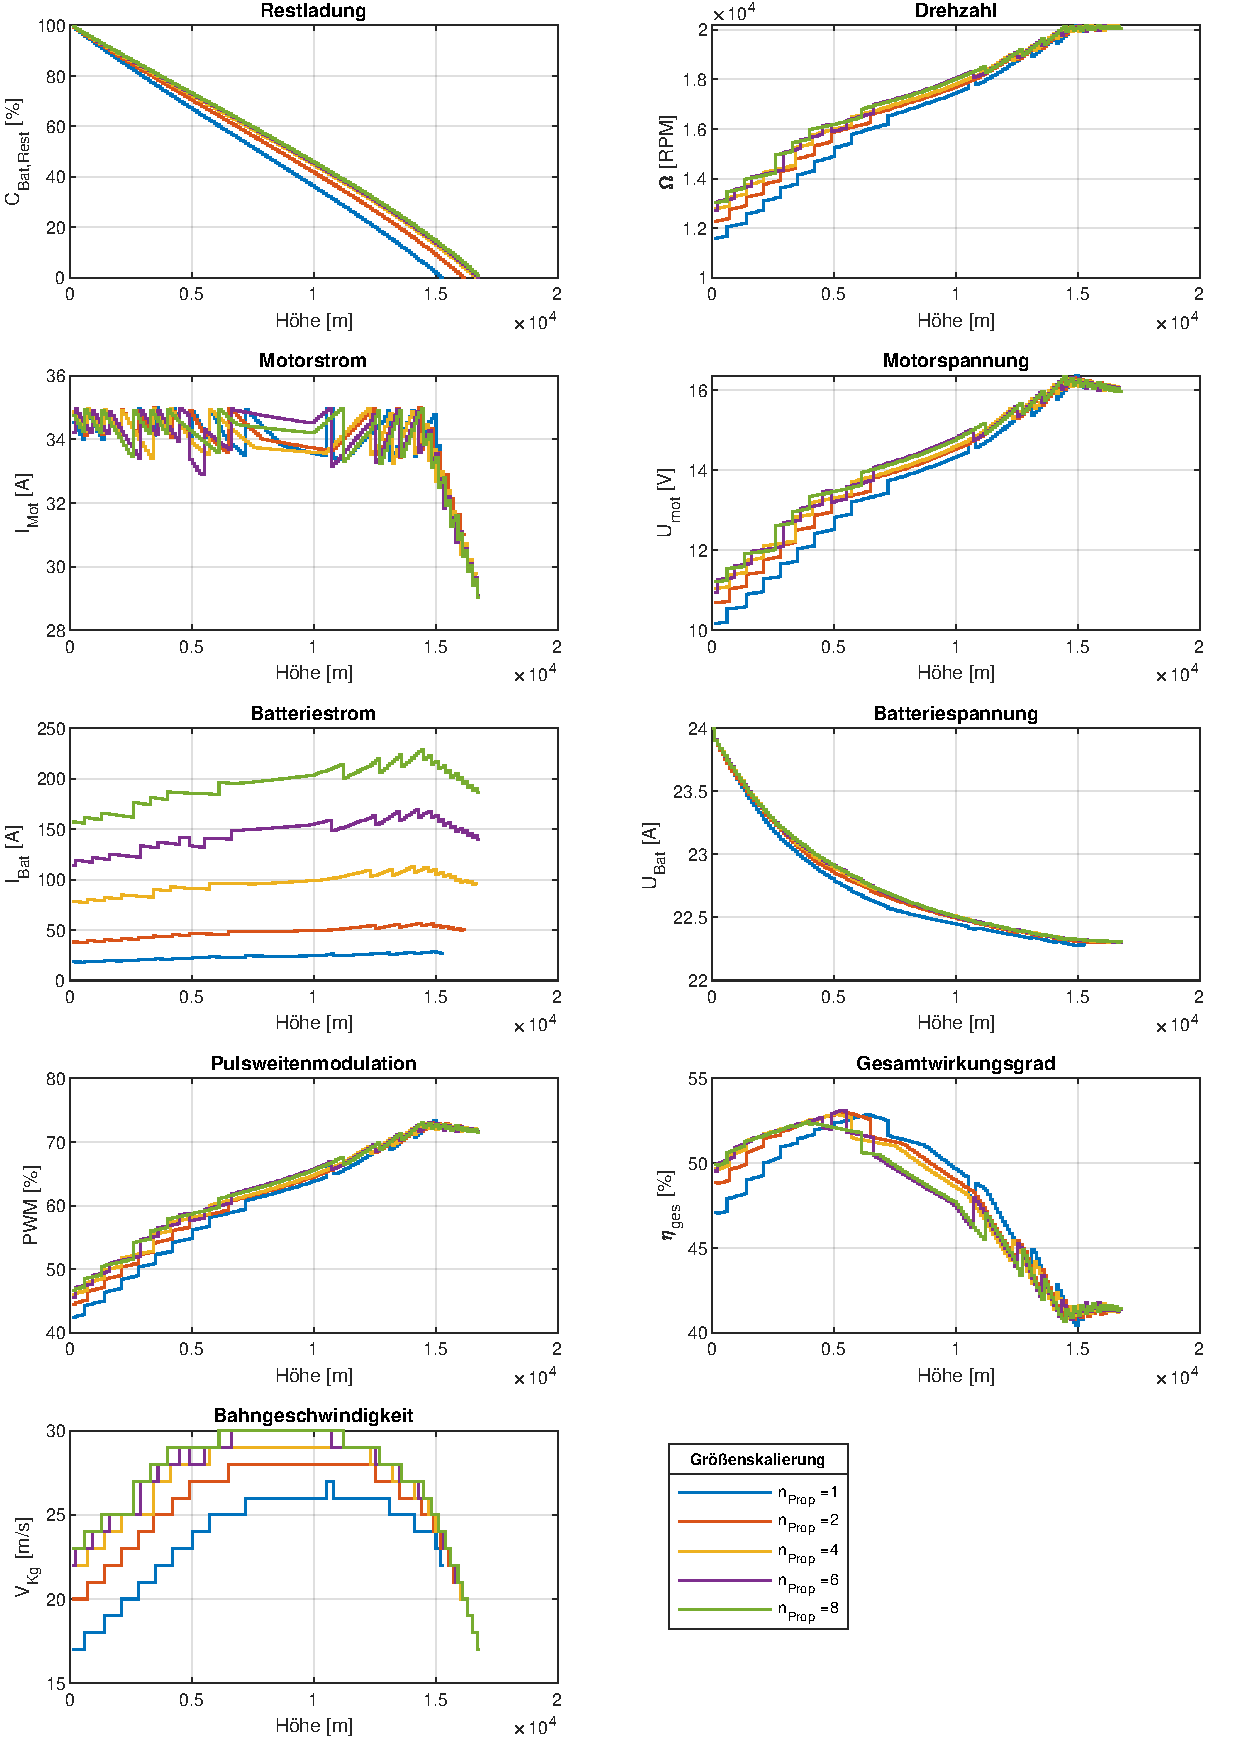
\includegraphics[scale=0.7]{Diagramme/Anz_Prop.pdf}
	\caption{Einfluss der Propelleranzahl auf die Flugleistungen der Multicopter-Referenzkonfiguration (Tab. \ref{tab:referenzkonfiguration_mulitcopter})}
	\label{abb:groessenskalierung}
\end{figure}
Analog zu den Ergebnissen aus Abschn. \ref{subsec:groesse} bewirkt eine äquivalente Veränderung der Rotoranzahl keine nennenswerten Änderungen der maximalen Flughöhe, wenn die verwendeten Motoren dieselben sind. Die Ergebnisse für einen Multicopter mit vier, sechs oder acht Propellern sind nahezu identisch. Dies gilt auch für die Restladung, die für diese Konfigurationen im Vergleich zu den Konfigurationen mit weniger Propellern noch pro Höhenschritt mehr Restladung aufweisen. Die einzigen Unterschiede weisen der Batteriestrom und die Bahngeschwindigkeit auf. Der Batteriestrom erhöht sich mit beinahe konstanten \SI{50}{A} pro zusätzlichen zwei Propellern (vgl. Gleichung \eqref{eq:batteriestrom}). Dahingegen steigt auch die Bahngeschwindigkeit mit mehr Propellern. \\
An dieser Stelle sind jedoch Einschränkungen vorzunehmen. 
Der Monocopter erreicht ähnliche Flugleistungen wie die anderen Konfigurationen. Der Monocopter benötigt jedoch zusätzlich noch Aktuatorik für die Abdeckung der restlichen drei Stellgrößen. Das umfasst Aktuatorik für das Nicken, Rollen und Gieren. Die translatorische Fortbewegung kann bereits durch den Propeller erfolgen. Der Drehmomentenausgleich könnte durch eine der drei rotatorischen Stellgrößen erfolgen (z.B. Rollen). Insgesamt sind also mindestens drei weitere Aktuatoren notwendig. Diese zusätzliche Aktuatorik benötigt der Duocopter ebenfalls. Ein Drehmomentenausgleich ist hier jedoch nicht notwendig. Trotzdem sind hier immerhin noch zwei weitere Aktuatoren für das Nicken und Gieren erforderlich. 
Beide erwähnten Punkte erhöhen die Gesamtmasse und benötigen zusätzlich Energie. Dies verringert die Gesamthöhe. 
Für mehr als vier Propeller muss berücksichtigt werden, dass die Gesamtmasse und damit insbesondere das Strukturgewicht steigt. Dies geht auf die Kosten einer optimalen Konstellation der Massenverteilung. Zusätzlich erhöht sich die obere Stirnfläche \ensuremath{F_{copter,oben}} durch stärkere Strukturen, die in einer Widerstandserhöhung und somit erhöhten Verlusten resultieren. 
Für den anschließenden Sinkflug wäre ein um die Gierachse eigenstabiler und um die Roll- und Nickachse mit den zusätzlichen zwei Aktuatoren steuerbarer Duocopter, welcher die beiden Antriebe abschaltet und sich somit im Gleichtflug befindet, womöglich sehr effizient. Diese Art der Konfiguration spricht für einen Gleitflüger, der die beiden genannten Eigenschaften verbindet.
Um das oben gesagte zusammenzufassen, eignet sich eine Propelleranzahl von mindestens zwei am besten für einen Flug in die untere Stratosphäre. \\


\subsection{Einfluss eines Verstellpropellers}
\label{subsec:verstellprop}
Eine bisherige Begrenzung der Flugleistungen erfolgte häufig durch die maximale Drehzahl des Propellers, die indirekt die Motorspannung beeinflusst (vgl. Abschn. \ref{subsec:widerstandseinfluss}). 
Besonders auffällig bei vorherigen Untersuchungen (vor allem in Bezug auf die Untersuchungen des Quadrocopters aus Kap. \ref{chap:nachbildung_des_quadrocopter}) ist, dass die Drehzahl von Propellern mit einer geringen Steigung deutlich schneller steigt als bei einem Propeller mit einer großen Steigung. Da vor allem die Drehzahl die Motorspannung bestimmt, ist eine Verringerung der Drehzahl bei gleichem Schub von Interesse. Mit zunehmender Flughöhe verringert sich die Dichte und dementsprechend auch der Schub, wenn die Rotordrehzahl und die Propellersteigung konstant gehalten werden. Diesem Effekt kann mit einer Erhöhung der Drehzahl oder mit einer Erhöhung der Steigung entgegen gewirkt werden. Während bei einem Drehflügler mit Strahltriebwerk nur eine Blattverstellung, nicht aber eine Drehzahlveränderung möglich ist, besitzen elektrische, propellergetriebene Fluggeräte beide Möglichkeiten. Dies kann mit einem Verstellpropeller und entsprechender Aktuatorik realisiert werden. \\
Im Rahmen dieser Untersuchung liegen nur Propellerkennfelder mit einer konstanten Propellersteigung vor. Das Vorgehen für einen Propeller mit variabler Steigung sieht so aus, dass für einen vorgegebenen Durchmesser alle Kennfelder mit diesem Durchmesser der Datenbank entnommen werden (siehe \ref{sec:vprop_vorgehen}). Danach wird in der Leistungsuntersuchung jeder Propeller mit unterschiedlicher Steigung, aber gleichem Durchmesser, gegeneinander abgewogen. Die Auswahl für den in dem betrachteten Flugmoment beste Steigung erfolgt wieder über die Energiebetrachtung analog zum Bahnneigungswinkel und der Bahngeschwindigkeit (vgl. Kap. \ref{subsubsec:schub_flaechenflzg}). Dies ist ein Idealfall, weil mit der minimal aufgebrachten Energie auch die der Batterie entzogenen Restladung minimal ist. Folglich wird nur der Zustand ausgewählt, der die größte Restladung aufweist.

\begin{figure}[H]
\centering
	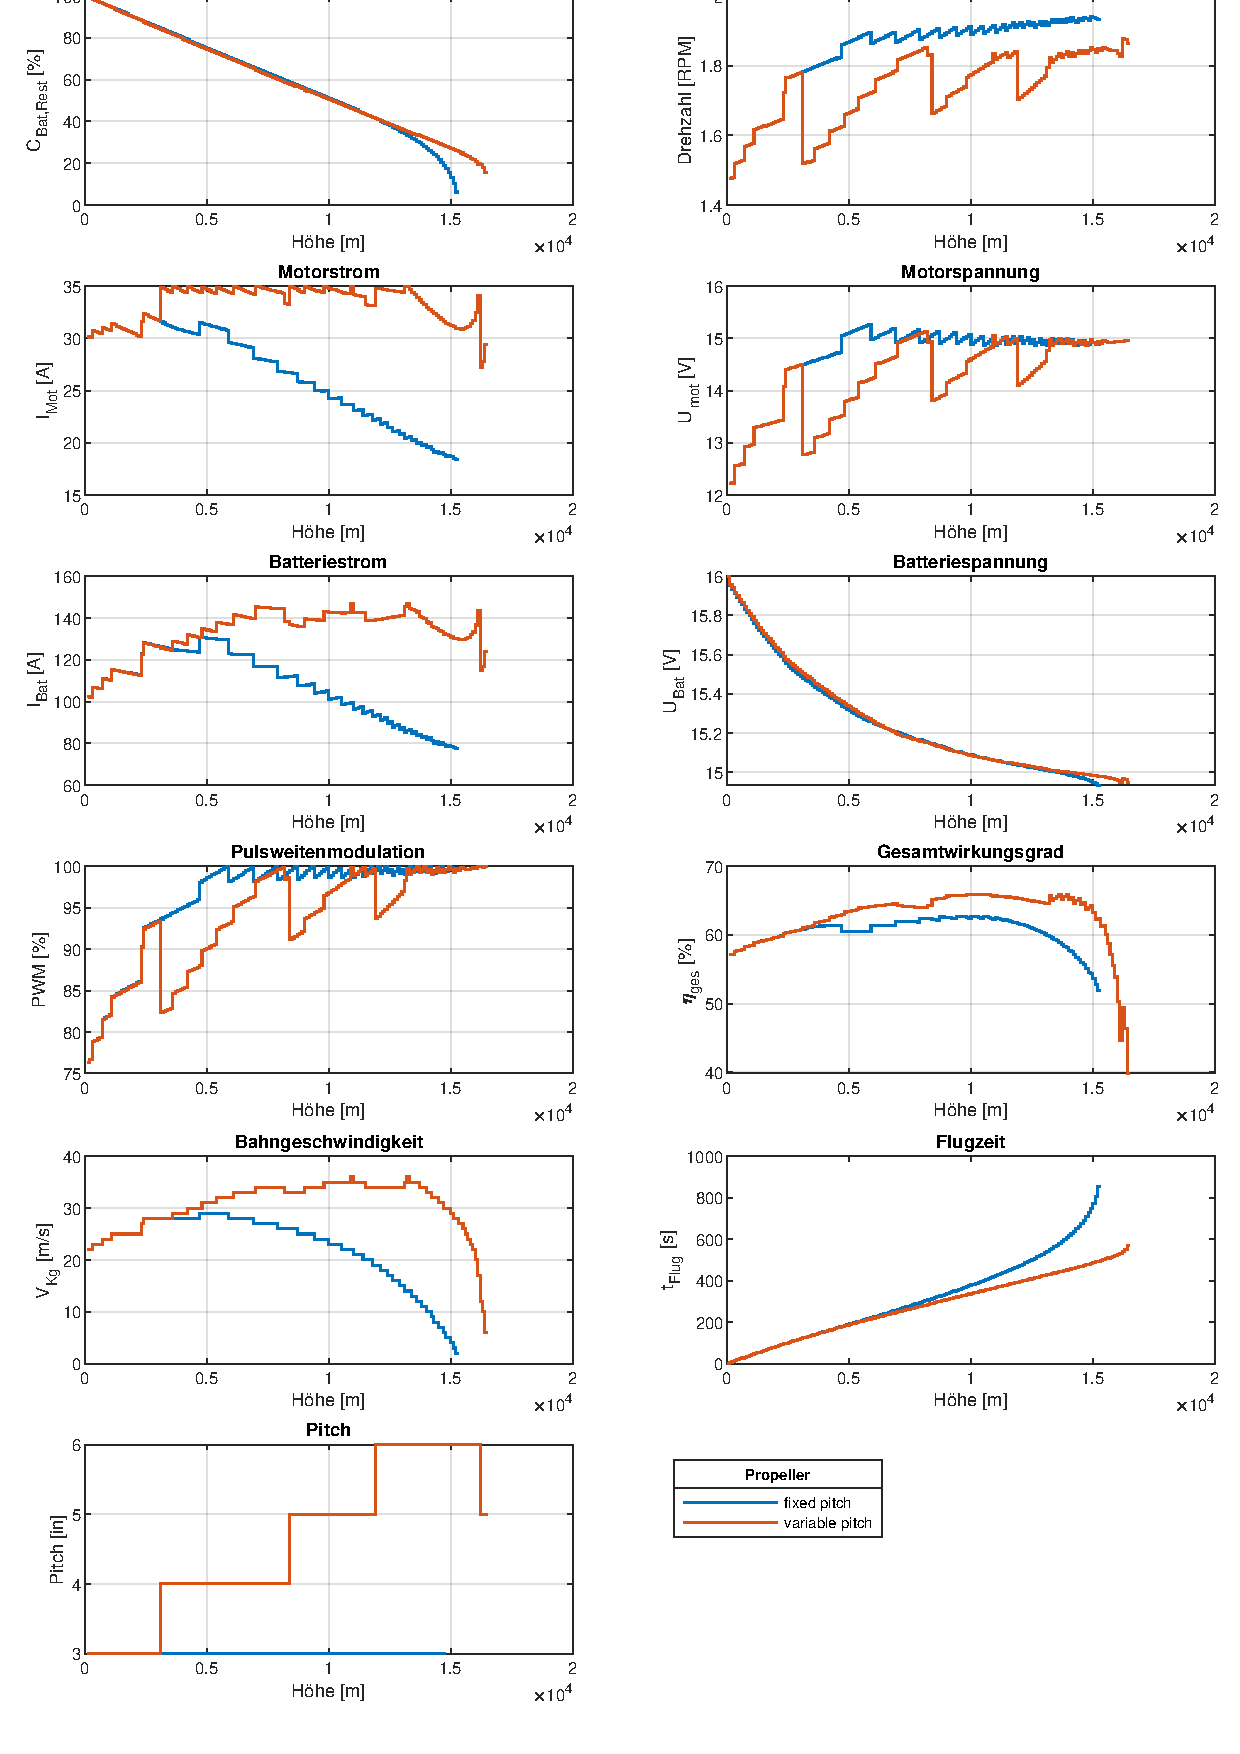
\includegraphics[scale=0.7]{Diagramme/Verstellpropeller.pdf}
	\caption{Einfluss eines idealen (Eigengewicht gleich null und ideale Verwindung) Verstellpropellers auf die Multicopter-Referenzkonfiguration (Tab. \ref{tab:referenzkonfiguration_mulitcopter})}
	\label{abb:verstellpropeller}
\end{figure}
Mit dem Verstellpropeller ist ein deutlicher Höhengewinn von \SI{2000}{m} zu verzeichnen. Selbst mit dem Verstellpropeller wird ab \SI{17500}{m} die Dienstgipfelhöhe erreicht, die sich wieder durch die Begrenzung der Propellerdrehzahl auszeichnet. Ab \SI{17000}{m} ist die Blattspitzengeschwindigkeit  \ensuremath{Ma_{tip} = 1}. Allerdings sind die Auswirkungen auf die Flugleistungen marginal. Hieraus kann geschlossen werden, dass ein Verstellpropeller die Dienstgipfelhöhe in größere Höhen verschieben kann. \\
Mit dem Verstellpropeller kann durchgehend am effizientesten bei maximalen Motorstrom (hier \ensuremath{I_{max} = \SI{35}{A}}) geflogen werden. Die Propellersteigung wächst im Laufe des Steigfluges von anfänglichen \SI{3}{in} auf \SI{5}{in}. Dies ist erstaunlich, da noch viel größere Steigungen möglich wären, die aber selbst in großen Flughöhen immer noch mehr Energie der Batterie entziehen als kleinere Steigungen. Es gilt also, dass geringe Propellersteigungen für Multicopter am effizientesten mit Hinblick auf den Energieverbrauch sind. Die Fluggeschwindigkeit ist allerdings auch gering, sodass sich hohe Steigungen tendenziell erst bei hohen Fluggeschwindigkeiten lohnen. \\
Signifikant ist der Einfluss einer Propellersteigungsänderung auf die Propellerdrehzahl. Aufgrund der Tatsache, dass der Verstellpropeller mit Kennfeldern von Propellern modelliert wird, die eine feste Steigung besitzen, bedeutet eine Änderung der Propellersteigung auch eine Änderung der Drehzahl. Diese Drehzahleinbrüche treten auf, da ein Propeller mit einer höheren Steigung denselben Schub bei einer geringeren Drehzahl erzeugen kann. Der Verlauf der Drehzahl wirkt sich direkt auf die Motorspannung aus (vgl. Gleichung \eqref{eq:motorspannung}), damit auch auf die PWM (vgl. Gleichung \eqref{eq:pwm}) und letztlich auf den Batteriestrom (vgl. Gleichung \eqref{eq:batteriestrom}). Im Vergleich zum Propeller mit konstanter Steigung ist die PWM durch die vergleichsweise geringere Drehzahl und die geringere Motorspannung unterhalb der PWM der Referenzkonfiguration. Folglich fällt auch der Motorreglerwirkungsgrad schlechter aus. Allerdings wird durch die Propellersteigungsänderung eine deutliche Erhöhung des Propellerwirkungsgrades erzielt. Dies kann auf die langsamer drehenden Propeller, aber deutlich schneller fliegenden Multicopter zurückgeführt werden (vgl. Gleichung \eqref{eq:eta_prop}). Eine Propellersteigungserhöhung liefert gleichzeitig auch mehr Schub. Somit ist auch eine höhere Bahngeschwindigkeit möglich. Insgesamt liegt somit der Gesamtwirkungsgrad \ensuremath{\eta_{ges}} vom Multicopter mit Verstellpropeller ab \SI{7000}{m}, wenn die Propellersteigung das erste Mal erhöht wird, ca. \SI{3}{\%} (mit einer steigenden Tendenz) über dem Multicopter ohne. In \SI{15000}{m} Höhe sind es sogar mehr als \SI{10}{\%}. \\
Eine Änderung auf die Abnahme der Restladung macht sich erst ab ca. \SI{10000}{m} Höhe bemerkbar. Während die Restladung vom Multicopter ohne Verstellpropeller ab dieser Höhe schneller abnimmt, kann sie durch einen Verstellpropeller verlangsamt werden. Dies bedeutet, dass ein Verstellpropeller die Effizienz in niedrigen Höhen nicht bedeutend beeinflusst. Für Steigflüge in großen Höhen kann er jedoch die Effizienz deutlich anheben.
% Dies gilt jedoch nicht bei Steigflügen in noch größere Höhen, da er dort die Effizienz deutlich anhebt.
%Der zusätzliche Höhengewinn durch einen Verstellpropeller liegt bei  ca. \SI{1500}{m} (vgl. Abb \ref{abb:verstellpropeller}). Dabei handelt es sich um einen idealen Verstellpropeller, dessen Verstellmechanismus und -aktuatorik nicht in das Gesamtgewicht einbezogen werden. \\
%Die Leistungsparameter beider Propellerarten sind für die ersten \SI{3000}{m} identisch. Dies liegt an der gleichen Propellersteigung. Danach nimmt die optimale Propellersteigung kontinuierlich zu. Durch die Tatsache, dass die Steigung variabel ist, ist durchgehend ein Flug mit maximaler Motorleistung, d.h. bei einem maximalen Motorstrom und -spannung, möglich. Durch jede Verstellung kommt es zu einem Einbruch der Drehzahl, der sich durch den Verlauf der Motorspannung und der PWM fortpflanzt (entspr. Gleichung \eqref{eq:motorspannung} und \eqref{eq:pwm}). Bis zu einer Höhe von \SI{3000}{m} hat der Verstellpropeller keinen Einfluss auf die Restladung oder die Batteriespannung. Die deutlich höhere Effizienz des Fluges bei maximalen Motorstrom zeigt sich im Gesamtwirkungsgrad. Durch die mit der Propellersteigungsänderung steigende Bahngeschwindigkeit erhöht sich auch der Propellerwirkungsgrad. Daher erhöht sich auch der Gesamtwirkungsgrad. 
%Ein Vorteil, der in Abb. \ref{abb:verstellpropeller} ersichtlich wird, ist, dass durch eine Erhöhung der Propellersteigung der gleiche, wenn nicht sogar noch mehr Schub, bei einer geringeren Drehzahl durch den Propeller erzeugt werden kann. Dies erhöht den Leistungsüberschuss und letztendlich die erreichbaren Fluggeschwindigkeiten bei voller Motorauslastung. Entsprechend sinkt die Flugzeit.
%Bedeutend ist noch zu erwähnen, dass die Restladung am TOC bei einem Multicopter mit Verstellpropeller noch bedeutend höher ist (insg. noch ca. \SI{20}{\%}) als die bei einem ohne. \\
Der Vorteil eines Verstellpropellers ist deutlich. Dazu müssen aber noch folgende Einschränkungen vorgenommen werden. Der Verstellpropeller kann nur im Rahmen der in der APC-Datenbank \cite{apc} vorhanden Propeller modelliert werden. Dies setzt Ungenauigkeiten voraus, da eine kontinuierliche Verstellung nicht nachgebildet werden kann und nur so viele Verstellungen berücksichtigt werden können, wie auch Propeller mit verschiedenen Steigungen in der Datenbank vorhanden sind. Eine kontinuierliche Verstellung würde an dieser Stelle einen glatten Verlauf in der Propellersteigung und somit auch in allen anderen Verläufen erzeugen. \\
An dieser Stelle wurde der Propeller in gewisser Weise idealisiert. So wurde unter anderem die verlängerte Blattaufhängung mit dem Steuerstangenanschluss und der Verstellaktuatorik etc. außer Acht gelassen. Dies würde zu zusätzlichen Verlusten an der Blattwurzel und einer Verringerung des effektiven Radius führen. Bei einem Propeller mit konstantem Anstellwinkel kann diese sehr kurz gehalten werden, weshalb das profilierte Rotorblatt radial gesehen deutlich früher beginnt. Die Verringerung der effektiven Propellerblattlänge ist bei dem hier modellierten Verstellpropeller nicht berücksichtigt worden. Weiterhin birgt die Verwendung von Propellerkennfeldern mit einer festen Steigung gewisse Ungenauigkeiten. Für die Propeller mit fester Steigung kann vorausgesetzt werden, dass dieser im Rahmen eines optimalen Schwebeflugrotors \cite[S.197-S.205]{Wall.2015} ausgelegt wurde (ausschließlich axiale Anströmung, Betrieb nur im Vorwärtsflug, etc). Ein Verstellpropeller muss jedoch eine gewisse Bandbreite an Betriebspunkten abdecken (Steig-, Vorwärtsflug oder Autorotation), die durch eine einseitige Optimierung des Propellers eine Verschlechterung für die anderen bedeutet \cite[S.203]{Wall.2015}. Es ist daher auch mit Diskrepanzen für das Leistungsverhalten des Verstellpropellers in Bezug auf Propeller mit fester Steigung zu rechnen, die nicht den Kennfeldern zu entnehmen sind. \\
Weiterhin wurden in dieser Betrachtung das Gewicht des Verstellmechanismus an sich und der Aktuatorik für jeden einzelnen Propeller nicht berücksichtigt. Hierbei bedeuten die Aktuatoren zusätzliche Verbraucher für die Batterie, die mitunter deutlich schneller zu einem Flug bei \SI{100}{\%} PWM führen würden. Letztendlich ist der fehlende Schub in großen Höhen nicht das Begrenzungsmerkmal, sondern die Drehzahl des Propellers und Motors sowie die Batteriespannung, kurz der Leistungsüberschuss. Letzterer macht den Verstellpropeller ein weiteres Stück redundant. %(vgl. \ref{abb:vertellprop_real}). 
Mit einem hohen Batteriestrom verschiebt sich der Bereich, in dem ein größere Steigung vorteilhafter ist, noch weiter in größere Höhen. Damit sinkt auch die Einsatzdauer und schließlich der Nutzen. 
Schlussendlich bringt der Verstellpropeller den Vorteil der Autorotation mit, der weniger für den Steigflug als für den anschließenden Sinkflug von Bedeutung ist. Durch die Autorotation ist ein antriebsloser Sinkflug möglich. Damit könnte die Batterie noch weiter entladen werden bevor ein Sinkflug eingeleitet werden muss, was im Umkehrschluss die erreichbare Höhe steigert. Außerdem erhöht ein Verstellpropeller die Restladung am TOC, sodass das volle Potential dieser Propellerart ausgeschöpft werden kann. Im Zustand der Autorotation ist jedoch kein Ausgleich von Seitenwinden möglich. Die Abdrift muss daher an dieser Stelle negativ bewertet werden. \\
Zusammengefasst gilt, dass ein Verstellpropeller Vorteile in großen Höhen mit sich bringt. Allerdings ist die hier in Abb. \ref{abb:verstellpropeller} dargelegte Effizienz anzuzweifeln. Die Vorteile ergeben sich auch in Abhängigkeit der Konstruktion. Je kleiner die Blattaufhängung ist, desto effizienter ist der Verstellpropeller. Weiterhin ist die Masse des Verstellmechanismus im Verhältnis zum Gesamtgewicht abzuwägen. Je größer das Gesamtgewicht des Multicopters, desto geringer ist der nachteilige Einfluss der Zusatzmasse durch den Verstellpropeller auf dessen Flugleistungen. Aus diesem Grund ist der reale Nutzen für kleinere Multicopter zu verneinen. 
In \ref{sec:vprop_vorgehen} werden die Flugleistungen für einen Verstellpropeller mit Eigengewicht dargelegt. 



\subsection{Einfluss eines stufenlosen Getriebes}
\label{subsec:getriebe}
Eine häufige Begrenzung der Leistung ist die maximale Drehzahl des Motors oder des Propellers (vgl. u.a. Abschn. \ref{sec:flaechenflugzeug_referenzkonfig} und \ref{subsec:widerstandseinfluss}). Diese nimmt mit großen Höhen stark zu. Ein hypothetisches, stufenlos verstellbares Getriebe bringt den Vorteile mit, dass durch dessen Einsatz die Drehzahl für den Motor entsprechend angepasst werden kann, sodass die Motorspannung nicht mehr den Flaschenhals für einen Steigflug darstellt.
Die Übersetzung für ein Getriebe 
\begin{equation}
	i = \frac{\Omega_{an}}{\Omega_{ab}} 
	\label{eq:getriebe_uebersetzung}
\end{equation}
setzt sich in Abhängigkeit der Drehzahlen aus dem Verhältnis der Eingangsdrehzahl \ensuremath{\Omega_{an}} zur Ausgangsdrehzahl \ensuremath{\Omega_{ab}} zusammen. Weiterhin gilt für die Leistung, dass unter Berücksichtigung von Verlusten innerhalb des Getriebes die Eingangsleistung \ensuremath{P_{an}} gleich der Ausgangsleistung \ensuremath{P_{ab}} ist
\begin{equation}
	P_{an} = \eta_{Getriebe} \cdot \Omega_{an}\cdot M_{an} = \Omega_{ab}\cdot M_{ab} = P_{ab}
	\label{eq:getriebe_leistung}
\end{equation} 
mit dem Getriebewirkungsgrad 
\begin{equation}
	\eta_{Getriebe} = \frac{P_{ab}}{P_{an}} \leq 1 \eqend{.}
	\label{eq:getriebe_wirkungsgrad}
\end{equation}
Aus den Gleichungen \eqref{eq:getriebe_uebersetzung} bis \eqref{eq:getriebe_wirkungsgrad} ergeben sich nun für die aus dem Propellerkennfeld ermittelten Drehzahl und dem Drehmoment die neue Drehzahl für den Motor
\begin{equation}
	\Omega_{neu} = \Omega_{Kennfeld}\cdot i
\end{equation}
und aus der Leistung
\begin{equation}
	M_{neu} = \frac{P_{ab}}{\Omega_{neu}} \eqend{.}
\end{equation}
das neue Drehmoment.
Die günstigste Übersetzung wird analog zum Steigwinkel des Flächenflugzeuges und analog zur Bahngeschwindigkeit durch eine Iteration über der Übersetzung \ensuremath{i} gefunden (siehe Anhang \ref{sec:getriebe_vorgehen}). Das Entscheidungskriterium ist auch hier die minimal aufgebrachte Energiemenge für den jeweiligen Höhenschritt. An dieser Stelle ist das Getriebegewicht \texttt{m\_Getriebe} nicht zu vernachlässigen. Diese fließt mit der Anzahl der Propeller in die Berechnung der Gesamtmasse mit ein
\begin{equation}
	m = m_{Bat} + (m_{Mot} + m_{Getriebe})\cdot n_{Prop} + m_{Copter} \eqend{.}
\end{equation}

\begin{figure}[H]
\centering
	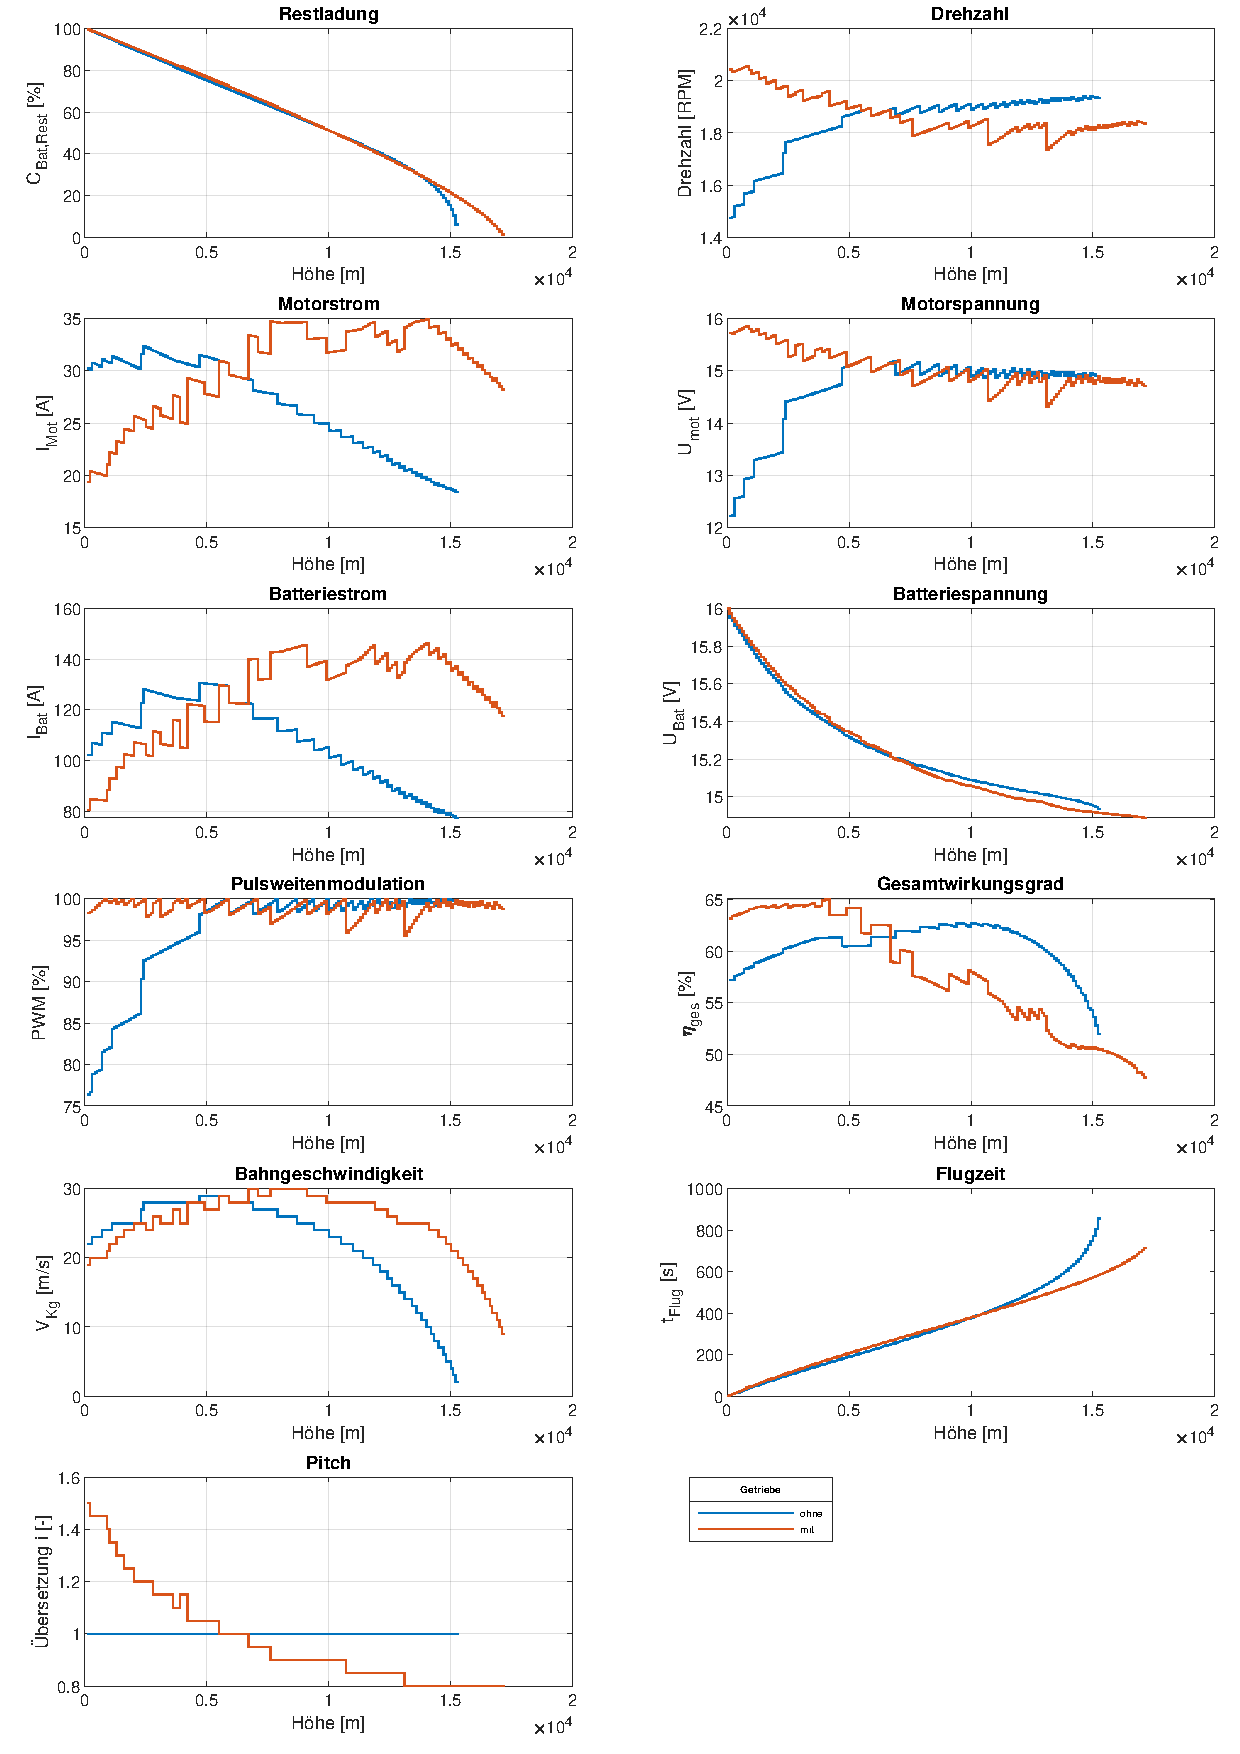
\includegraphics[scale=0.7]{Diagramme/Getriebe.pdf}
	\caption{Einfluss eines idealen (Eigengewicht gleich null und Getriebewirkungsgrad gleich \SI{100}{\%}) Getriebes auf die Flugleistungen der Multicopter-Referenzkonfiguration (Tab. \ref{tab:referenzkonfiguration_mulitcopter})}
	\label{abb:getriebe}
\end{figure}
Der Einsatz eines idealen, stufenlosen Getriebes (\ensuremath{m_{Getriebe} = 0} und \ensuremath{\eta_{Getriebe} = 1}) bietet nur minimale Vorteile (vgl. Abb. \ref{abb:getriebe}). Durch das Getriebe ist die Restladung im Durchschnitt um \SI{2}{\%} größer als ohne. Aus der Reihenfolge des Programms ist die Übersetzung der Drehzahlen und Drehmomente genau umgekehrt. In diesem wird die Drehzahl des Propellers für den Motor angepasst. Mit dieser Blickweise wird die Motordrehzahl zuerst ins Schnelle übersetzt und anschließend ab ca. \SI{15000}{m} Höhe ins Langsame. Auf Grund der Tatsache, dass die Leistung über einem Getriebe konstant bleibt und hier vorerst keine weiteren Verluste berücksichtigt werden, ist der Verlauf des Drehmoments komplementär zu dem Drehzahl, sodass die Beziehung in Gleichung \eqref{eq:getriebe_leistung} erhalten bleibt. \\
Die Übersetzung hat keinen Einfluss auf die Propellerdrehzahl. Diese wird durch Interpolation aus dem Propellerkennfeld bestimmt (vgl. Kap. \ref{subsec:propellerzustand}). Die bemerkbaren Unterschiede in Abb. \ref{abb:getriebe} ergeben sich durch die Diskretisierung der Getriebeübersetzung.
Ähnlich kleine Unterschiede weist auch die Bahngeschwindigkeit auf. Dementsprechend klein sind auch die Unterschiede in der Flugzeit. Das stufenlose Getriebe übersetzt hauptsächlich die Drehzahl des Propellers derart, dass der Motor eine beinahe konstante Spannung erfährt von ca. \SI{17}{V}. Die Motorspannung sinkt dabei leicht mit der Höhe auf \SI{16}{V}. Verantwortlich für die konstante Motorspannung ist die Übersetzung, die beinahe hyperbolisch von anfangs 2 auf 0,9 abnimmt. Der Motorstrom ist durch die Übersetzung des Drehmoments zu Beginn bei \SI{17}{A} und steigt kontinuierlich auf \SI{35}{A}, dem maximalen Motorstrom \ensuremath{I_{max}}. Entsprechend zur Motorspannung bleibt auch die PWM konstant bei ca. \SI{74}{\%}. Dies kennzeichnet einen effizienten Flugzustand, der sich durch einen höheren Gesamtwirkungsgrad \ensuremath{\eta_{ges}} im Gegensatz zur Referenzkonfiguration auszeichnet.

\begin{figure}[H]
\centering
	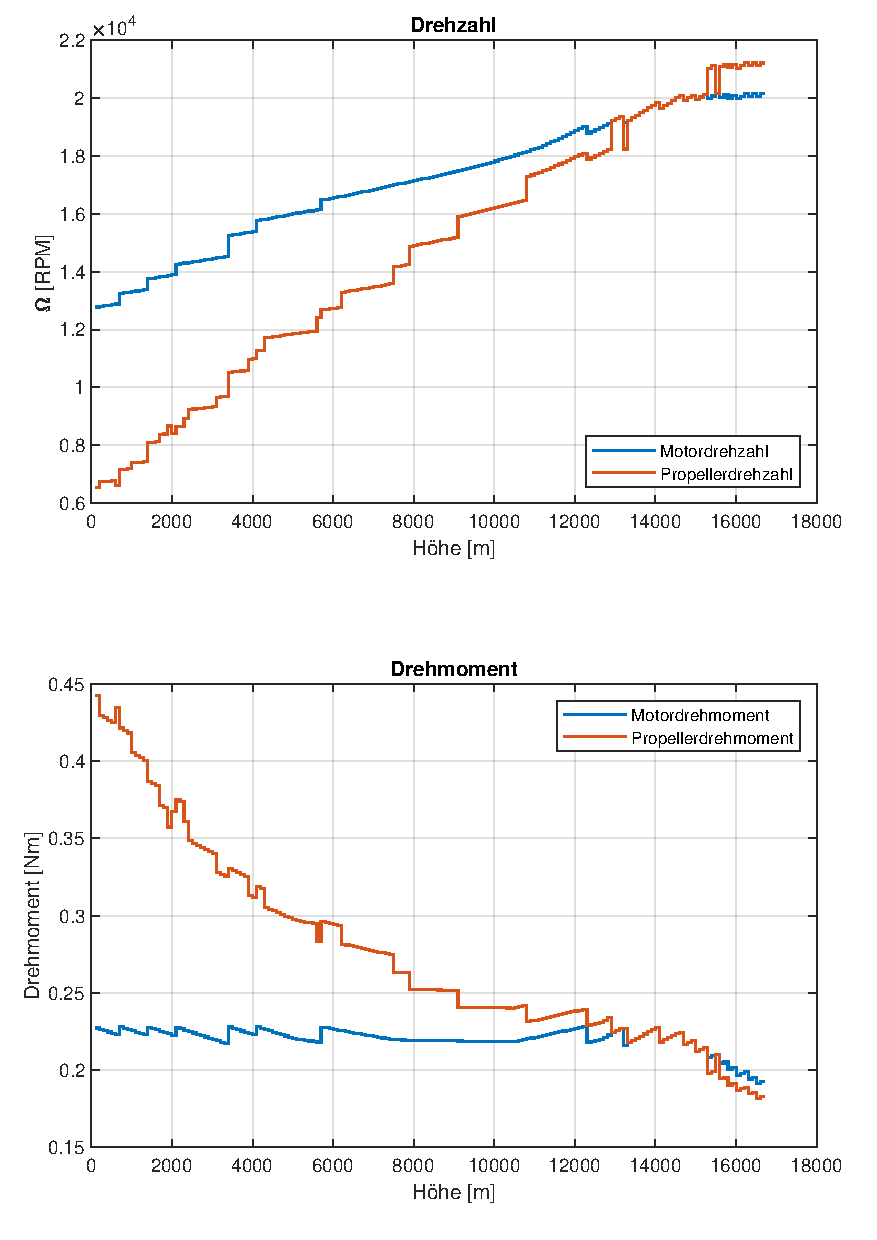
\includegraphics[scale=0.5]{Diagramme/Drehzahl_und_Drehmoment.pdf}
	\caption{Auswirkungen der Übersetzung des Getriebes auf die Drehzahl und das Drehmoment von Motor und Propeller}
	\label{abb:getriebe_dud}
\end{figure}

In der Realität besitzt ein stufenloses Getriebe oder CVT-Getriebe jedoch immer ein Eigengewicht und zeichnet sich durch einen vergleichsweise schlechten Wirkungsgrad aus \cite[S.295-S.297]{Fischer.2016}. %(\SI{0.8}{} zu etwa \SI{0.95}{} bei einem Stufengetriebe)
Die hohen Verluste können auf die hohe erforderliche Reibkraft und Verstellkraft zurückgeführt werden. Unter Berücksichtigung dieser verringert sich der Höhengewinn schrittweise, je größer das Getriebegewicht und dessen Verluste ausfallen. 
Zusätzlich ist anzuzweifeln, dass stufenlos verstellbare Getriebe im Modellbau existieren, die ein sehr geringes Eigengewicht besitzen und sich daher für Flugmodell eignen.
Das Gewicht eines einzelnen Getriebes beläuft sich dabei auf mehr als \SI{750}{g} \cite{cvt}, wobei die Verstellelektronik nicht berücksichtigt wurde. Für einen vierrotorigen Multicopter entspräche das einem Zusatzgewicht von mehr als \SI{3000}{g}. 
Die Vorteile eines CVT-Getriebes werden durch dessen Nachteile deutlich überkompensiert. Ein solches Getriebe bedeutet bei all seiner Kampaktheit und Effizienz letztendlich große Zusatzmasse und einen weiteren, verlustbehaftete Komponenten innerhalb der Antriebskette. Aus all diesen Gründen kann von dem Einsatz eines stufenlosen Getriebes für einen Multicopter abgesehen werden.


\section{Vorschlag einer optimalen Lösung}
\label{sec:otimale_lsg}
Aus den bisherigen Parameteruntersuchung soll nun eine optimale Konfiguration vorgestellt werden (vgl. Abschn. \ref{subsec:vorueberlegung}). Anschließend erfolgt die Darstellung der Flugleistungen unter idealen Randbedingungen (vgl. Abschn. \ref{subsec:ideale_rb}) und danach unter den Randbedingungen, die im AEROMET\_UAV-Projekt vorgegeben sind (vgl. Abschn. \ref{subsec:aeromot_rb}). 


\subsection{Vorüberlegungen}
\label{subsec:vorueberlegung}
Für den Antrieb ist ein Motor mit hohem \ensuremath{K_V}-Wert zu wählen, der zusätzlich wenige interne Verluste hat (vgl. Abschn. \ref{subsec:mot_prop_kombi}). In Bezug auf den gewählten Motor ist der Propeller auszuwählen. Eine Minimierung der aerodynamischen Verluste trägt zu einer Effizienzsteigerung bei (vgl. Kap. \ref{subsec:widerstandseinfluss}). Einen großen Einfluss auf die Flugleistungen hat die Batterie. Kurz zusammengefasst sollte die Batteriemasse einen Anteil von 2/3 der Gesamtmasse einnehmen (vgl. Kap. \ref{subsec:massenverteilung}). Dabei ist die Batteriezellenanzahl in Bezug auf den Motor festzulegen (vgl. Kap. \ref{subsec:einfluss_n_bat}).
Die optimale Anzahl der Propeller liegt zwischen vier und acht Propellern (vgl. Kap. \ref{subsec:anz_prop}). Es gibt kaum Unterschiede in den Flugleistungen dieser Konfigurationen. Ein Verstellpropeller bringt gewisse Vorteile mit, die die Dienstgipfelhöhe und den anschließenden Sinkflug betreffen. Allerdings werden diese durch die zusätzlichen Verluste überkompensiert (vgl. Kap. \ref{subsec:verstellprop}). Dies betrifft ebenso den hypothetischen Einsatz eines stufenlos verstellbaren Getriebes (vgl. Kap. \ref{subsec:getriebe}). \\
Die optimale Konfiguration ist in Tab. \ref{tab:optimale_konfiguration} konkretisiert.

\begin{center}
	\captionof{table}{wichtige Parameter der optimalen Multicopter-Konfiguration}
	\begin{tabular}{l l l} \hline
		Parameter & Variablenname & verwendete Größe \\ \hline
		Gesamtmasse \ensuremath{m} & \texttt{m} & \SI{3,504}{kg} \\
		Leermasse des Multicopters \ensuremath{m_{copter}}& \texttt{m\_copter} & \SI{1.028}{kg} \\ 
		Batteriemasse \ensuremath{m_{Bat}} & \texttt{m\_Bat} & \SI{2,052}{kg} \\
		Motormasse \ensuremath{m_{Mot}}& \texttt{m\_Mot} & \SI{106}{g} \\
		Geschwindigkeitskonstante \ensuremath{K_V} & \texttt{K\_V} & \SI{1390}{RPM/V} \\
		maximaler Dauerstrom \ensuremath{I_{max}} & \texttt{I\_max} & \SI{35}{A} \\
		Propeller & \texttt{prop\_name} & 11x4 \\
		Anzahl Propeller \ensuremath{n_{Prop}} & \texttt{n\_prop} & \SI{4}{} \\ 
		Anzahl der Batteriezellen \ensuremath{N_{Bat,cell}} & \texttt{N\_bat\_cell} & 5 \\	 
		Obere Stirnfläche \ensuremath{F_{copter,oben}} & \texttt{F\-copter\_oben} & \SI{0,0209}{m^2} \\
		Oberer Widerstandsbeiwert \ensuremath{c_{W,copter,oben}} & \texttt{c\_W\_copter\_oben} & 0,5 \\ \hline
	\end{tabular}	
	\label{tab:optimale_konfiguration}
\end{center}
Änderungen im Vergleich zu der Multicopter-Referenzkonfiguration (vgl. Tab. \ref{tab:referenzkonfiguration_mulitcopter}) ergeben sich unter anderem in der Batterie. Die Batteriezellenanzahl ist um eine Zelle verringert und die Batteriemasse auf einen Anteil von 2/3 an der Gesamtmasse erhöht worden. Weiterhin wird dem Quadrocopter eine aerodynamische günstige Form zugesprochen, weshalb der oberer Widerstandsbeiwert sich auf \SI{0,5}{} reduziert. Im Sinne einer Effizienzsteigerung wird auch die Propellersteigung um \SI{1}{in} erhöht, sodass der Propeller für die optimale Konfiguration ein 11x4 Propeller ist. Die letzte vorgenommene Änderung betrifft den Wirkungsgrad der Motorregler. An dieser Stelle wird davon ausgegangen, dass sich die Verluste innerhalb des Reglers halbieren. Die Leermasse, die obere Stirnfläche und die Motoren ändern sich nicht.


\subsection{Ideale Randbedingungen}
\label{subsec:ideale_rb}
Für die Untersuchung unter idealen Randbedingungen ist die Windgeschwindigkeit auf \SI{10}{m/s} gesetzt (vgl. Kap. \ref{sec:multicopter_referenzkonfig}) und es wird zusätzlich keine  Nutzlast mitgeführt.
Die bestmögliche Konfiguration erreicht eine Höhe von  mehr als \SI{18000}{m} (vgl. Abb. \ref{abb:optimale_konfig}). Auch dieses Mal erreicht die Konfiguration ihre Dienstgipfelhöhe, welche sich durch ein Absinken der Bahngeschwindigkeit ab \SI{12100}{m} gegen \SI{0}{m/s} auszeichnet. Der Grund für die Bahngeschwindigkeitsabnahme ist die limitierte Antriebsleistung. Sie ist am Ende der ausschlaggebende Parameter. Deutlich zu erkennen ist, dass die Motoren bereits zu Beginn des Fluges mit maximalem Motorstrom betrieben werden. Hier lassen sich zwei Gründe ausmachen.
Der Erste betrifft den Propeller. Der Propeller zeigt mit seinen \SI{11}{in} Durchmesser eine hohe Effizienz wie der TOC, die Restladung und der Propellerwirkungsgrad verdeutlichen. Jedoch bedeutet ein großer Propellerdurchmesser auch gleichzeitig ein hohes Propellerdrehmoment, was im Umkehrschluss einen hohen Motorstrom folgert (vgl. Gleichung \eqref{eq:motorstrom}). Deshalb wird der Propellerschub durch den maximalen Motorstrom von \SI{35}{A} limitiert. Rückwirkend wirkt sich dies auf die Bahngeschwindigkeit aus, die damit nach oben begrenzt ist. \\
Der zweite Grund umfasst das Gesamtgewicht. Die insgesamt \SI{3,504}{kg} Gesamtmasse stellen ein hohes Gewicht dar und gleichzeitig eine hohe Schubanforderung (vgl. Gleichung \eqref{eq:schub_multicopter}). Ähnlich zum Propeller erzeugt der hohe, benötigte Schub wieder einen großen Motorstrom. \\
Beide Gründe verursachen einen hohen Motorstrom, der eine Abriegelung der Motorleistung auf \ensuremath{I_{max}} erforderlich machen. Dem schließt sich eine Begrenzung der Bahngeschwindigkeit an. \\
Deutlich zu erkennen ist, dass der Motor jedoch nicht bei \SI{100}{\%} PWM betrieben wird. In diesem Sinne ist noch ein Leistungsüberschuss gegeben.
Die Batterie weist auf der Höhe von \SI{15000}{m} noch mehr als \SI{40}{\%} Restladung auf (vgl. Abb. \ref{abb:optimale_konfig}). Mit dieser Restladung ist somit im Anschluss an den Steigflug noch ein sicherer Sinkflug möglich. Das Fluggerät kann wieder unbeschadet landen.

\begin{figure}[H]
\centering
	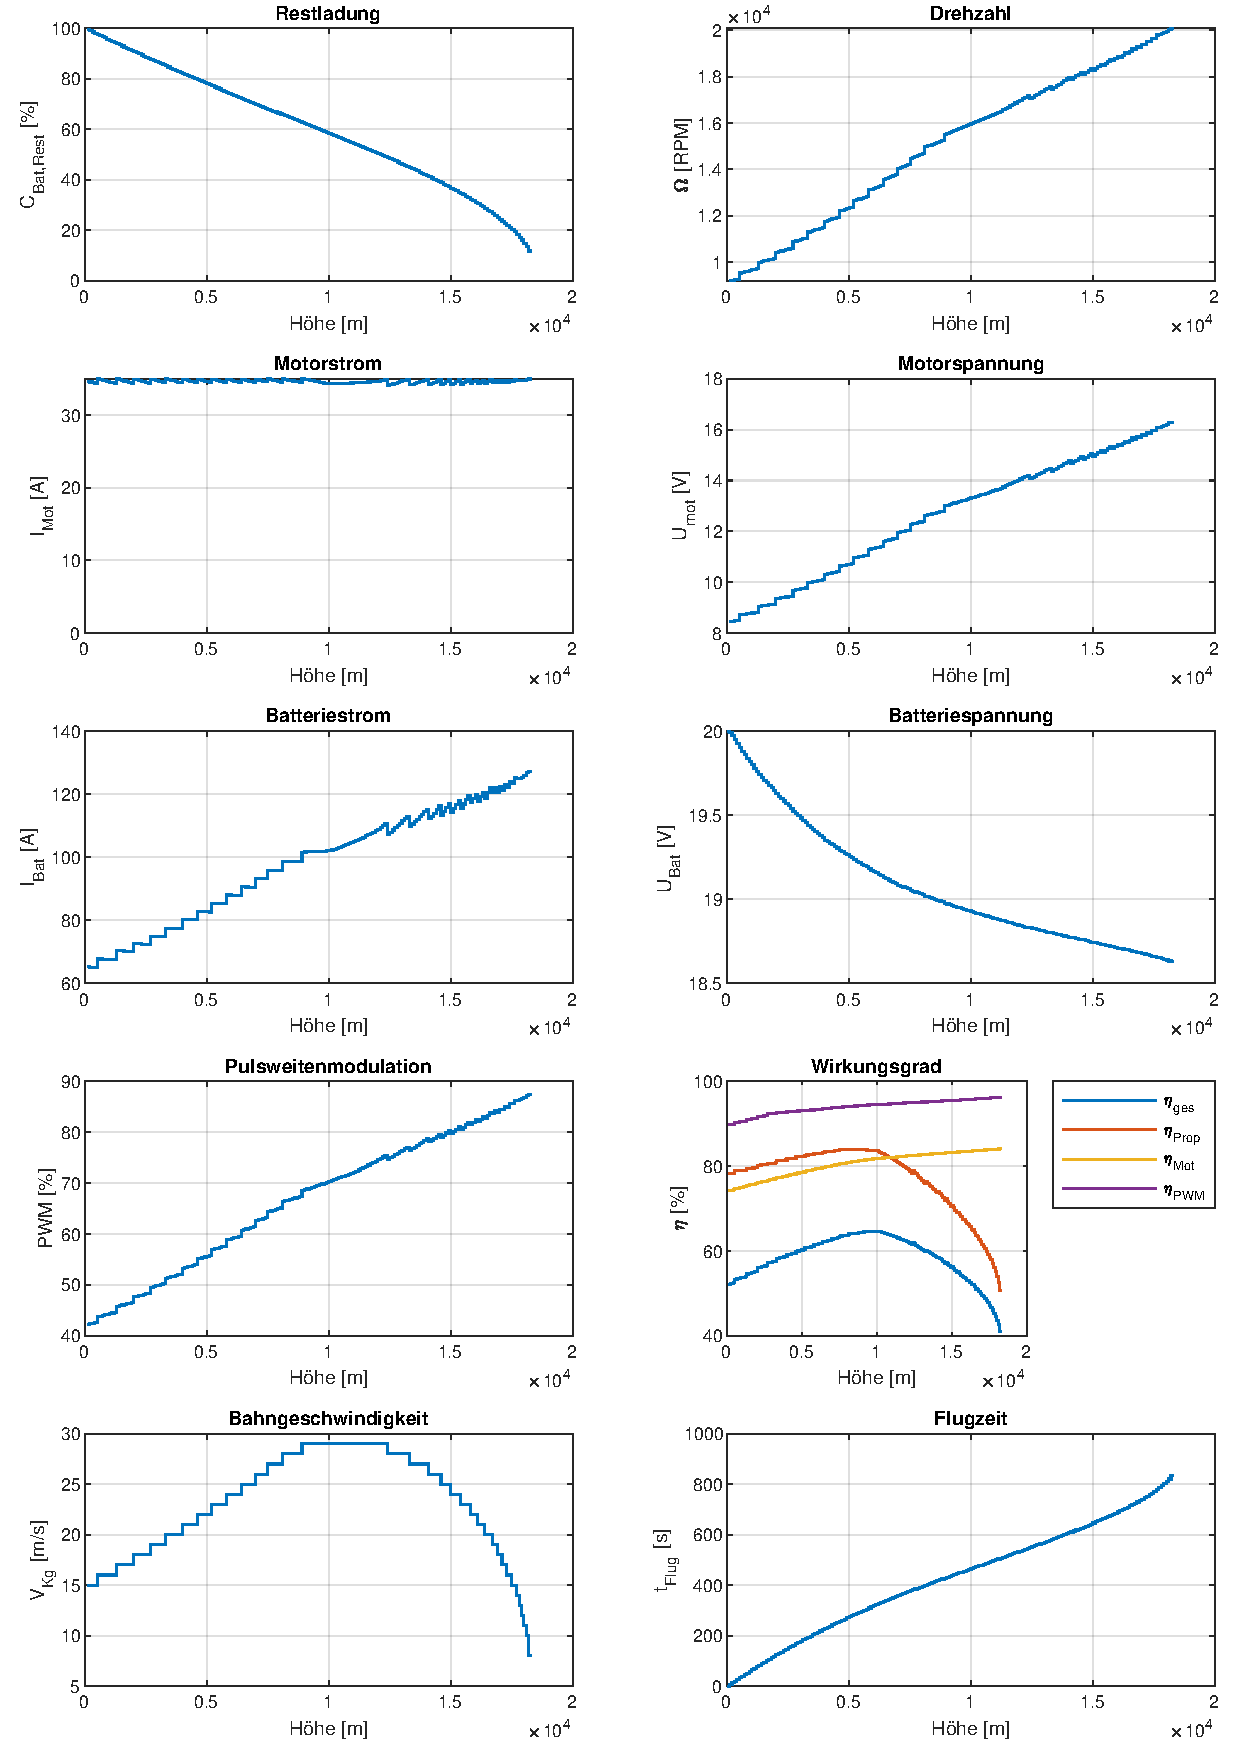
\includegraphics[scale=0.7]{Diagramme/Endergebnis.pdf}
	\caption{Die Flugleistungen der bestmöglichen Konfiguration (Tab. \ref{tab:optimale_konfiguration})}
	\label{abb:optimale_konfig}
\end{figure}



\subsection{AEROMET\_UAV Randbedingungen}
\label{subsec:aeromot_rb}
Schlussendlich soll noch der Einfluss der für dieses Projekt definierten Randbedingungen festgehalten werden. Die für das Projekt vorgeschriebenen Randbedingungen sind in Tab. \ref{tab:randbedingungen} aufgelistet. 
 
\begin{center}
\captionof{table}{wichtige Parameter des Flächenflugzeugs}
\begin{tabular}{l l l} \hline
	Parameter & Variablenname & verwendete Größe \\ \hline
	Windgeschwindigkeit \ensuremath{u_{Wg}} & \texttt{u\_Wg} & \SI{100}{km/h}\\
	Nutzlast \ensuremath{m_{Nutz}} & \texttt{m\_Nutz} & \SI{250}{g}  \\ \hline
\end{tabular}	
\label{tab:randbedingungen}
\end{center}

Erste Untersuchungen mit der optimalen Lösung aus Abschn. \ref{subsec:ideale_rb} haben ergeben, dass unter den AEROMET\_UAV-Randbedingungen maximal eine Höhe von \SI{8000}{m} erreicht werden kann. Hierbei wurde die Nutzlast auf die Gesamtmasse addiert. \\
Es existiert eine deutliche Korrelation zu den Aussagen in Abschn. \ref{subsec:ideale_rb}.\\
Durch das Zusatzgewicht der Nutzlast erhöht sich die Gesamtmasse zusätzlich. Damit steigt wiederum die Schubanforderung und letztlich der Motorstrom für jeden Höhenschritt. Dadurch erfolgt eine Abriegelung der Antriebsleistung schon bei geringen Bahngeschwindigkeiten und übrigen Leistungsparametergrößen. \\
Mit Bezug auf Abschn. \ref{subsec:propeller} und \ref{subsec:ideale_rb} ist eine Anpassung des Propellers vorzunehmen. Trotz der höheren Effizienz von größeren Propellerdurchmessern ist eine Verringerung dieses Parameters im Sinne einer Senkung des Propellerdrehmoments erforderlich. \\
Aus diesen Gründen sind kleine Änderungen an der optimalen Konfiguration vorzunehmen. Der Propellerdurchmesser wird um einen Inch verkleinert, sodass anstatt eines 11x4 ein 10x4 Propeller zum Einsatz kommt. Eine Reduzierung der Batteriemasse durch die Nutzlast erfolgt vorerst nicht. Der Zusammenhang wird im Folgenden und im Anhang \ref{sec:einfluss_nutzlast} genauer dargelegt.

\begin{figure}[H]
\centering
	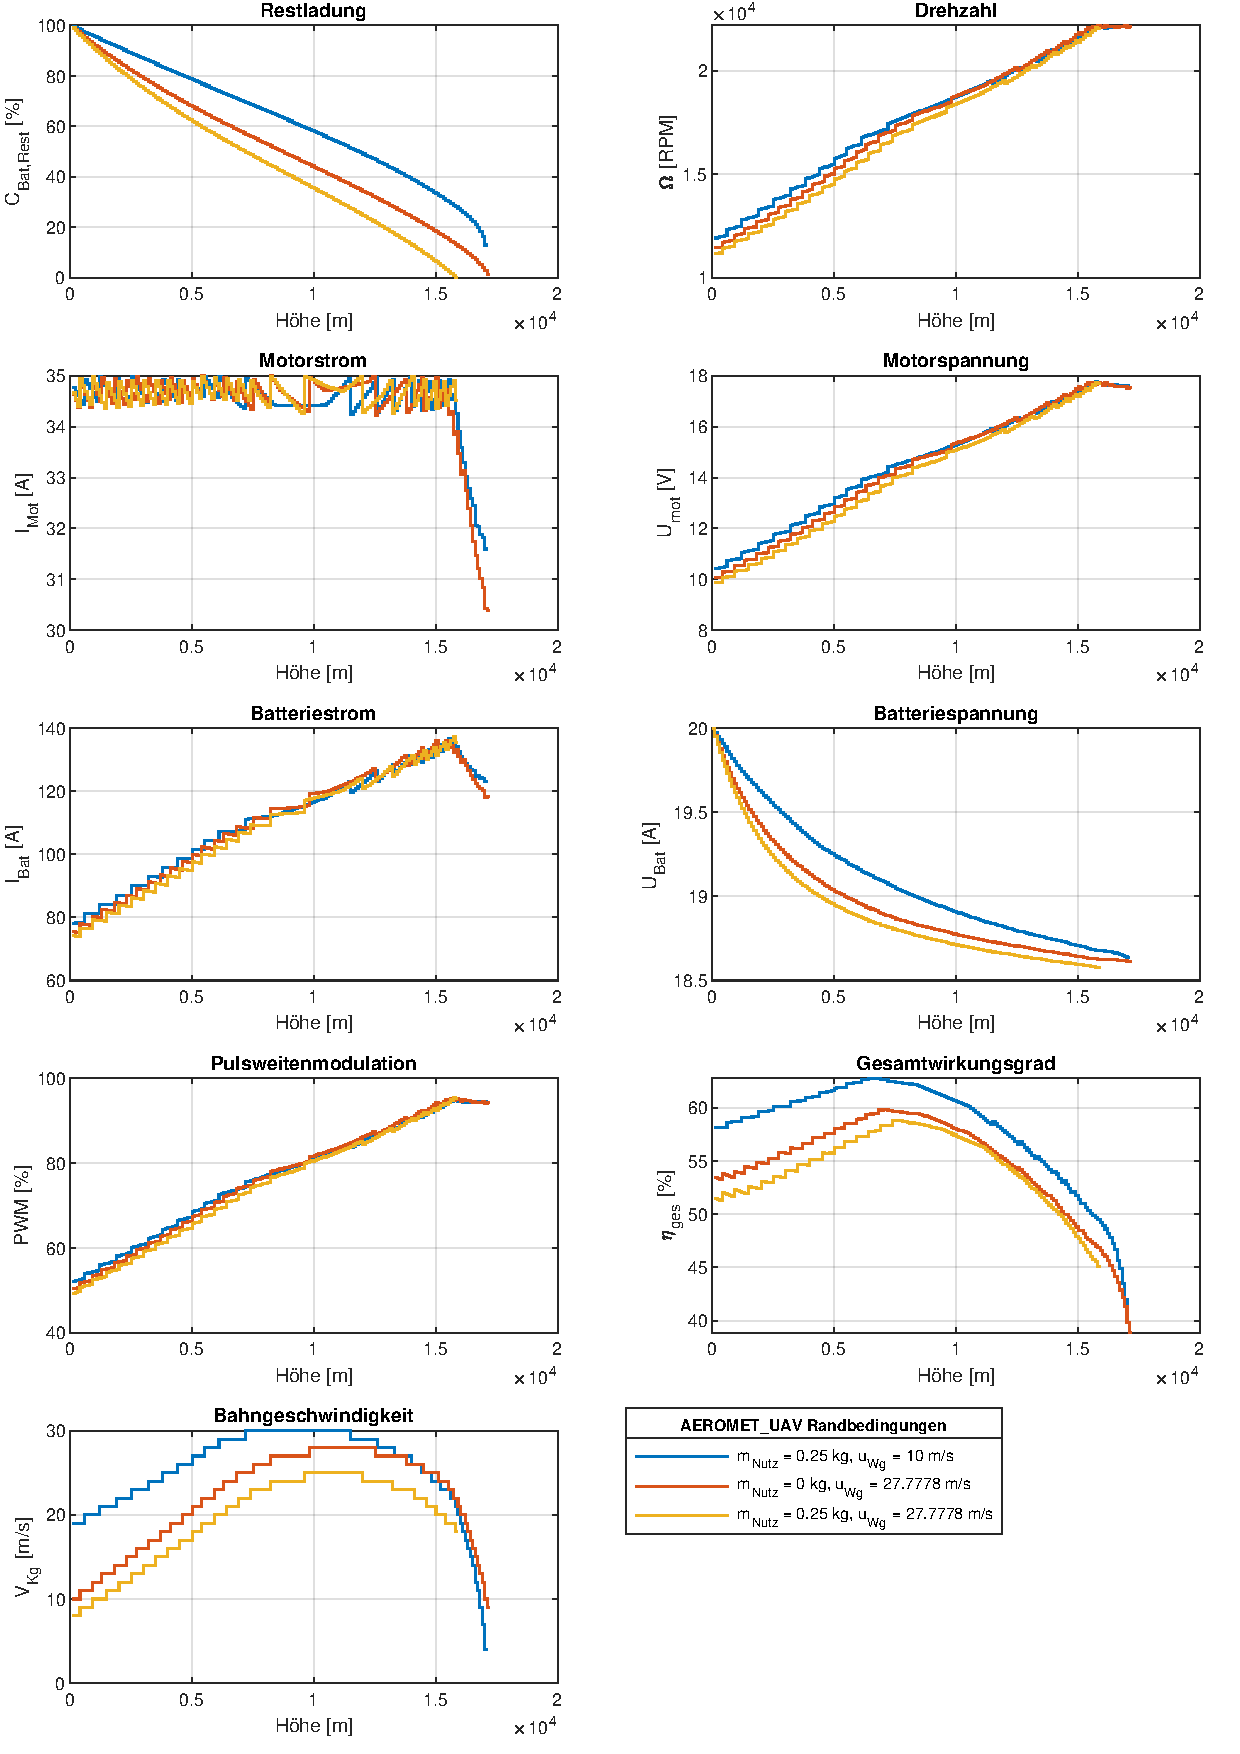
\includegraphics[scale=0.7]{Diagramme/aeromet_randbedingungen.pdf}
	\caption{Einfluss der AEROMET\_UAV-Randbedingungen auf die bestmögliche Konfiguration (Tab. \ref{tab:optimale_konfiguration})}
	\label{abb:aeromet_rb}
\end{figure}

Die Konfigurationen, die jeweils nur eine der Randbedingungen berücksichtigen, steigen beide bis zu ihrer Dienstgipfelhöhe auf. Diese liegt auf ca. \SI{18000}{m} Höhe (vgl. Abb. \ref{abb:aeromet_rb}). Der limitierende Parameter ist erneut die Propellerdrehzahl, die ab \SI{16000}{m} Höhe in den Bereich von einer Blattspitzengeschwindigkeit bei \ensuremath{Ma_{tip} = 1} kommt. Die Dienstgipfelhöhe verdeutlicht erneut die Notwendigkeit einer optimalen Propellerauswahl (vgl. Abschn. \ref{subsec:propeller} und \ref{subsec:vorueberlegung}). \\
Der Einfluss von \ensuremath{m_{Nutz}} ist im Vergleich zu der optimalen Konfiguration (vgl. Abschn. \ref{abb:optimale_konfig}) gering. Trotz der Verwendung eines kleineren Propellers beträgt die Differenz der Restladung z.B. auf \SI{15000}{m} Höhe gerade einmal \SI{4}{\%}. Anders ist der Einfluss der Seitenwindgeschwindigkeit. Diese verursacht einen starken Einbruch der Restladung bereits zu Beginn des Steigfluges (vgl. Abb. \ref{abb:aeromet_rb}). Im Laufe des Fluges ist die Batterierestladung im Durchschnitt ca. \SI{20}{\%} unterhalb des Restladungsverlauf der optimalen Konfiguration (vgl. Abb. \ref{abb:optimale_konfig}). Die Tendenz der Diskrepanzvergrößerung ist steigend.\\
Der Einfluss des Seitenwindes ist also bedeutend größer als der der Nutzlast. Je stärker der Seitenwind ist, desto größer ist der Energieaufwand zur Kompensation der Abdrift durch eine Neigung der Rotorebene. Diese Energie steht nun nicht mehr für einen Steigflug zur Verfügung. Folglich sinkt die Bahngeschwindigkeit und damit auch der Propellerwirkungsgrad \ensuremath{\eta_{prop}}. Dasselbe gilt für den Gesamtwirkungsgrad \ensuremath{\eta_{ges}}. \\
Das wirken beider Randbedingungen aus Tab. \ref{tab:randbedingungen} kommt einer Superposition des Nutzlasteinflusses und des Seitenwindeinflusses gleich. Die maximal erreichbare Flughöhe wird nochmals reduziert. Letztendlich können Flughöhen von \SI{15200}{m} erreicht werden. Die Restladung der Batterie verzeichnet eine schnellere Abnahme und der Gesamtwirkungsgrad ist am geringsten, was ebenso für die Bahngeschwindigkeit gilt. 

\subsection{Zusammenfassung}
\label{subsec:ergebnisse}
Die optimale Lösung aus aus Abschn. \ref{subsec:vorueberlegung} zeigt gute Flugleistungen, die noch eine ausreichende Restladung auf Dienstgipfelhöhe und somit einen anschließenden, sicheren Sinkflug gewährleistet. \\
Die Motoren werden durch den großen Propellerdurchmesser unter Idealbedingungen am oberen Leistungslimit durch den maximalen Motorstrom betrieben (vgl. Abschn. \ref{subsec:ideale_rb}). Dieser Zustand ist jedoch nachteilig für das Mitführen einer zusätzlichen Nutzlast und bei einem Flug mit höheren Seitenwinden. Eine Reduzierung des Propellerdurchmessers schafft Abhilfe. Weiterhin ist der Einfluss von starken Seitenwinden bedeutend größer als der der Nutzlast. Ein Verschlechterung der Flugleistungen durch deren kleiner Massenanteil an der Gesamtmasse ist begrenzt.\\
Ist der Quadrocopter zusätzlich mit aerodynamischen Vorrichtungen versehen, kann ein Gleitflug nach dem Erreichen des TOC eingeleitet werden, der nur noch einen wenig Energie beansprucht. Der Punkt vor dem zwingenden Einleiten des Sinkflugs verschiebt sich damit in noch größere Flughöhen.
